\documentclass[8pt]{mpscheatsheet}
\usepackage{amsmath, amssymb, mathtools, empheq, physics}
\usepackage{xcolor}
%\usepackage[table]{xcolor}
\usepackage{graphicx, tikz}
\usepackage{setspace}
\usepackage{inputenc}

\raggedcolumns

\usepackage[hidelinks,
            pdftex,
            pdfauthor={Marc Bischof},
            pdftitle={Analysis I/II},
            pdfcreator={}]{hyperref}

\author{\href{https://n.ethz.ch/\~mabischof}{Marc Bischof} - mabischof@student.ethz.ch}
\title{Analysis I/II}

% !TeX root = ../ZF_bmicha_Ana.tex
\newcommand{\cbreak}{%
    \vfill\null\columnbreak%
}
\newcommand{\mathbox}[2][]{%
    \begin{center}%
        \boxed{#2} #1
    \end{center}%
}

\renewcommand{\labelitemi}{%
    $\triangleright$%
}

\renewcommand{\div}{%
    \mathrm{div}
}

\newcommand{\rot}{%
    \mathrm{rot}
}

\renewcommand{\grad}{%
    \mathrm{grad}
}

\newcommand{\vvec}{%
    \vec{v}
}

\newcommand{\wvec}{%
    \vec{w}
}

\newcommand{\rvec}{%
    \vec{r}
}

\newcommand{\nvec}{%
    \vec{n}
}

\newcommand{\novec}{%
    \vec{n}_o
}

\newcommand{\dxt}{%
    \dot{x}
}

\newcommand{\ddxt}{%
    \ddot{x}
}

\newcommand{\dyt}{%
    \dot{y}
}

\newcommand{\ddyt}{%
    \ddot{y}
}

\setcounter{secnumdepth}{4}

\begin{document}

     \section{Funktionen}
        % !TeX root = ../../ZF_bmicha_Ana.tex
\subsection{Folgen und Reihen \texorpdfstring{\hfill S.38+51}{S.38+51}}  
    \begin{description}
        \item[beschränkt:] Alle Glieder sind in \emph{endlich breitem}, \emph{waagerechten Parallelstreifen} enthalten.
        \item[monoton wachsend:] $\quad a_{n+1} \leq a_n \qquad  (\emph{strikt}:\,\, <)$
    \end{description}
    \fbox{mon. wachsend/ fallend \& beschränkt $\Rightarrow$ konvergent}
    \subsubsection{Rechenregeln für konvergente Folgen}
        Falls $\displaystyle \lim_{n\to \infty} a_n = a$ und $\displaystyle \lim_{n\to \infty} b_n = b$, gilt:
        \begin{align*}
            \lim_{n \to \infty}(a_n \pm b_n) &= a \pm b\\
            \lim_{n \to \infty}(a_n \cdot b_n) &= a \cdot b\\
            \lim_{n \to \infty}(a_n / b_n) &= a / b.
        \end{align*}
    % \subsubsection{Geometrische Reihe}
    % \vspace{-1em}
    %     $$
    %         \sum_{n}^{\infty}a \cdot q^n = \frac{a}{1-q}, \quad \abs*{q} < 1
    %     $$
        % !TeX root = ../../ZF_bmicha_Ana.tex
\subsection{Asymptoten}
    Wir nennen eine Funktion $g(x)$ eine Asymptote von $f(x)$ für $x \to \infty$ falls
    $$
        \lim_{x \to \infty} (f(x) - g(x)) = 0.
    $$
        % !TeX root = ../../ZF_bmicha_Ana.tex
\subsubsection{Landau Symbol}
    \vspace{-0.5em}
    \begin{align*}
        \fbox{$f(x) = o(g(x)) \textrm{ für } x \to a$} &\Longleftrightarrow \lim_{x \to a} \frac{f(x)}{g(x)} = 0\\[0.5em]
        \fbox{$f(x) = O(g(x)) \textrm{ für } x \to a$}  &\Longleftrightarrow \lim_{x \to a} \left\lvert\frac{f(x)}{g(x)}\right\rvert \leq A \in \mathbb{R}
    \end{align*}
    \subsubsubsection{Es gilt:}
        \begin{align*}
            x^k = o(e^x) \quad &\textrm{ für } x \to \infty, \quad k \in \mathbb{R}\\
            \ln(x) = o(x^k) \quad &\textrm{ für } x \to \infty, \quad k > 0
        \end{align*}
        % !TeX root = ../../ZF_bmicha_Ana.tex
\subsection{Eigenschaften \texorpdfstring{\hfill S.54}{S.54}}
    Eine Funktion $f : A \to B$ ist eine Vorschrift, die jedem $x \in A$ ein Element $f(x) \in B$ zuordnet, $f: x \to f(x)$.
    \begin{description}
        \item[Definitionsbereich:] $D(f) = A$
        \item[Zielbereich:] $Z(f) = B$
        \item[Wertebereich:] $W(f) = \{ f(x) \vert \ x \in D(f)\}$   
    \end{description}
    
    \textit{Hinweis: Lücken im Defintionsbereich müssen bei der Diskussion der Stetigkeit nicht betrachtet werden.\\ Bsp:}
    \small{$$ f(x) = \frac{1}{x} \hspace{8pt} \textrm{ist in} \hspace{8pt} \mathbb{R} \setminus \{-1, 1 \} \hspace{8pt} \textrm{stetig}$$}
    
    \subsubsubsection{Surjektiv}\vspace{3pt}
    
        Jeder Wert im Zielbereich $Z(f)$ wird angenommen.
        
        \mathbox{
            W(f) = Z(f)
        }
    \begin{samepage}
         \subsubsubsection{Injektiv}\vspace{3pt}
        Jede Horizontale schneidet den Graphen $\Gamma(f)$ höchstens einmal.
        \begin{itemize}
            \item $f(x_1) = f(x_2) \Rightarrow x_1 = x_2$, sonst nicht injektiv
        \end{itemize}
    \end{samepage}
        
    \subsubsubsection{Bijektiv}\vspace{3pt}
    
        \begin{center}
            Injektiv \& Surjektiv $\Leftrightarrow$ Bijektiv $\Leftrightarrow$ Umkehrbar
        \end{center}
    \subsubsubsection{Inverse Funktion}\vspace{3pt}
    
        Sei $f(x)$ eine Funktion von $D(f)$ nach $W(f)$, dann ist $f^{-1}: W(f) \to D(f)$ mit $y \mapsto f^{-1}(y)$ die inverse Funktion von $f(x)$.
        \begin{itemize}
            \item $W(f^{-1}) = D(f)$
            \item $D(f^{-1}) = W(f)$
        \end{itemize}
    \subsubsubsection{Gerade \& Ungerade}%\vspace{3pt}
        \begin{description}
            \item[gerade:]\phantom{as} $f(-x) = f(x)$ 
            \item[ungerade:] $f(-x) = -f(x)$ 
        \end{description}
    \subsubsubsection{Stetigkeit}\vspace{3pt}
    
        $f(x)$ ist stetig im Punkt $\xi$ falls
        $$
            \lim_{x\to\xi^-} f(x) = f(\xi) = \lim_{x\to\xi^+} f(x).
        $$
        \begin{itemize}
            \item Bei Lücken in $D(f)$ werden die einzelnen Abschnitte separat betrachtet.
        \end{itemize}
        
    \subsubsubsection{Monotonie}\vspace{3pt}
    
        \textbf{(Strikt) Monoton Steigend}
            \begin{itemize}
                \item $x_1 < x_2\ \Longleftrightarrow\ f(x_1) \leq f(x_2)$ \hfill (strikt: $<$)
                \item $f'(x) \geq 0$ \hfill (strikt: $>$)
            \end{itemize}
        \textbf{(Strikt) Monoton Fallend}
            \begin{itemize}
                \item $x_1 < x_2\ \Longleftrightarrow\ f(x_1) \geq f(x_2)$ \hfill (strikt: $>$)
                \item $f'(x) \leq 0$ \hfill (strikt: $<$)
            \end{itemize}
    \subsubsubsection{Beschränktheit}\vspace{3pt}
    
        Alle Funktionswerte sind in einem endlich breiten waagerechten Parallelstreifen enthalten.


    \cbreak
    \section{Differentialrechnung}
        % !TeX root = ../../ZF_bmicha_Ana.tex
\subsection{Evolute \texorpdfstring{\hfill S.66}{S.66}}
    Parametrisierung der Krümmungsmittelpunkte an die Kurve $\rvec = (x(t), y(t))^T$.
    $$
        E(t) = 
        \begin{pmatrix}
            x_E(t)\\y_E(t)
        \end{pmatrix}
    $$
    \begin{align*}
        x_E(t) &= x - \frac{\dyt \left( \dxt^2 + \dyt^2 \right)}{\dxt \ddyt - \ddxt \dyt}\\[0.25em]
        y_E(t) &= y + \frac{\dxt \left( \dxt^2 + \dyt^2 \right)}{\dxt \ddyt - \ddxt \dyt}
    \end{align*}\vspace{3pt}
    
    Ortsvektor $\Vec{r}_M(t_o)$ des Krümmungsmittelpunkt mit gegebener Krümmung $k(t)$ \textit{$\rightarrow$ 2.2} und Normalenvektor $\Vec{n}(t_o)$ der Kurve an der Stelle $t_o$:
    
    $$ \Vec{r}_M(t_o) = \Vec{r}_o - \frac{\Vec{n}(t_o)}{|\Vec{n}(t_o)|} \cdot k(t) $$
    
    \vspace{3pt}
    
    mit $\Vec{n}(t_o) = \begin{pmatrix}
        \Dot{y}(t_o) \\ -\Dot{x}(t_o) 
    \end{pmatrix}$

        % !TeX root = ../../ZF_bmicha_Ana.tex
\subsection{Krümmung \texorpdfstring{\hfill S.66-67}{S.66-67}}
\vspace{3pt}

    \begin{itemize}
        \item Parametrisierung $\rvec(t) = (x(t),y(t))^T$
            $$
                k(t) = \frac{\dxt \ddyt - \ddxt \dyt}{\left( \dxt^2 + \dyt^2 \right)^{\frac{3}{2}}}
            $$
        \item Daraus folgt für die Parametrisierung $y = f(x)$:
        $$
            k(x)= \frac{f''(x)}{(1+f'(x)^2)^{3/2}}
        $$
        \item Polar-Parametrisierung $ \rho = f(\phi)$
            $$
                k(\phi) = \frac{(f(\phi))^2 + 2(f'(\phi))^2 - f(\phi) f''(\phi)}{[(f(\phi))^2 + (f'(\phi))^2]^{3/2}}
            $$
        
    \end{itemize}

    \vspace{5pt}
    
    \textit{$|k(t)|$ wird kleiner für abnehmende Krümmung d.h. grösserer Abstand zwischen Kurve und 
    Evolute.}
    \cbreak
    \section{Integralrechnung \texorpdfstring{\hfill S.70}{S.70}}
        % !TeX root = ../../ZF_bmicha_Ana.tex
\subsection{Bogenlänge \texorpdfstring{\hfill S.75}{S.75}}
    \begin{itemize}
        \item explizit $y = f(x)$
            $$
                l = \int_a^b \sqrt{1 + \left( f'(x) \right)^2} \ dx
            $$
        \item Polarkoordinaten $\rho = \rho(\varphi)$
            $$
                l = \int_{\varphi_1}^{\varphi_2} \sqrt{\rho^2 + \dot{\rho}^2} \ d\varphi
            $$
        \item Parametrisierung $\rvec(t) = (x(t),y(t))^T$
            $$
                l = \int_{t_1}^{t_2} \left\lvert \sqrt{\dxt^2 + \dyt^2} \right\rvert \ dt
            $$
    \end{itemize}
        % !TeX root = ../../ZF_bmicha_Ana.tex
\subsection{Uneigentliche Integrale}\vspace{3pt}

    \begin{center}
        Konvergiert $\Longleftrightarrow$ Grenzwert existiert
    \end{center}
    
    \subsubsubsection{1. Gattung}\vspace{3pt}
    
            Zu integrierende Funktion ist an der Grenze nicht definiert. Bsp.:
            $$
                \int\limits_{0}^{1}  \frac{1}{x} \ dx = \lim_{\xi \to 0^+} \int\limits_{\xi}^{1} \frac{1}{x} \ dx
            $$
    \subsubsubsection{2. Gattung}\vspace{3pt}
    
        Unendlicher Integrationsbereich. Bsp.:
        $$
            \int\limits_{0}^{\infty}  f(x) \ dx = \lim_{\xi \to \infty}\int\limits_{0}^{\xi} f(x) \ dx
        $$
    \subsubsection{Tricks}
        \vspace{-0.5em}
        $$
            \int\limits_{0}^{\infty}  \frac{1}{x^\alpha} \ dx  \qquad \text{konvergiert} \iff \alpha > 1       
        $$
        % !TeX root = ../../ZF_bmicha_Ana.tex
\subsection{Flächenberechnungen \texorpdfstring{\hfill S.75}{S.75}}
    \textit{Hinweis: Für die Lösunge folgender Formeln muss der Betrag genommen werden, da eine Fläche immer positiv sein muss.}
    
    \vspace{0.5em}
    \begin{itemize}
        \item Parametrisierung $\rvec=(x(t),y(t))^T$ \hfill
    \end{itemize}
    \begin{minipage}{0.65\linewidth}
        \vspace{-1em}
        \begin{itemize}
        \item[]  $\displaystyle A= \int_{t_1}^{t_2} y \dxt \, dt$
        \item[] $x(t)$ monoton
        \item[]
        \end{itemize}
    \end{minipage}
    \begin{minipage}{0.34\linewidth}
        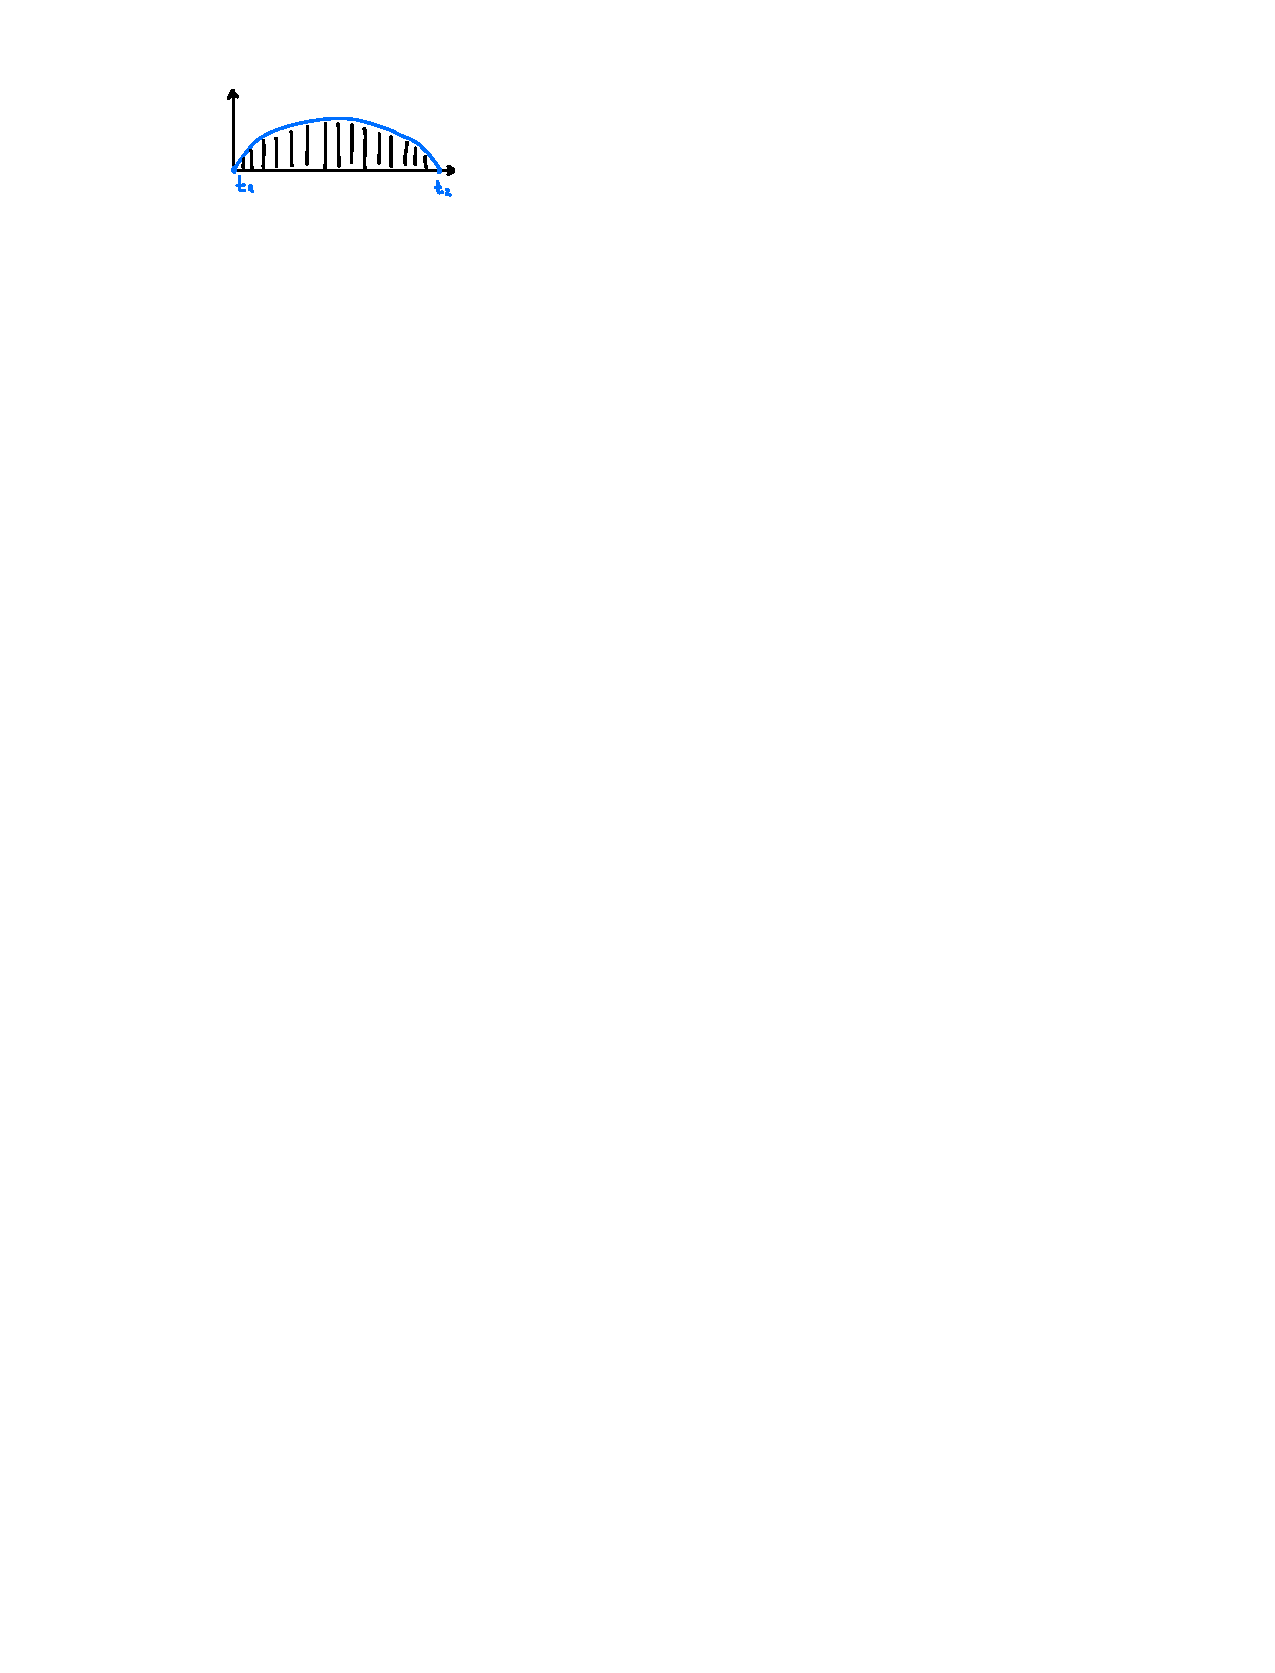
\includegraphics[width=0.7\linewidth]{src/Integralrechnung/param.pdf}
    \end{minipage}
    \begin{minipage}{0.65\linewidth}
        \begin{itemize}
            \item Sektorfläche
            \item[]  $\displaystyle A= \frac{1}{2} \int_{t_1}^{t_2} (x \dyt - y \dxt) \, dt$ 
            \item[] $t\mapsto (x(t),y(t))$ injektiv auf $(t_1,t_2)$ und stetig diff'bar
            \end{itemize}
            \item[]
    \end{minipage}
    \begin{minipage}{0.34\linewidth}
            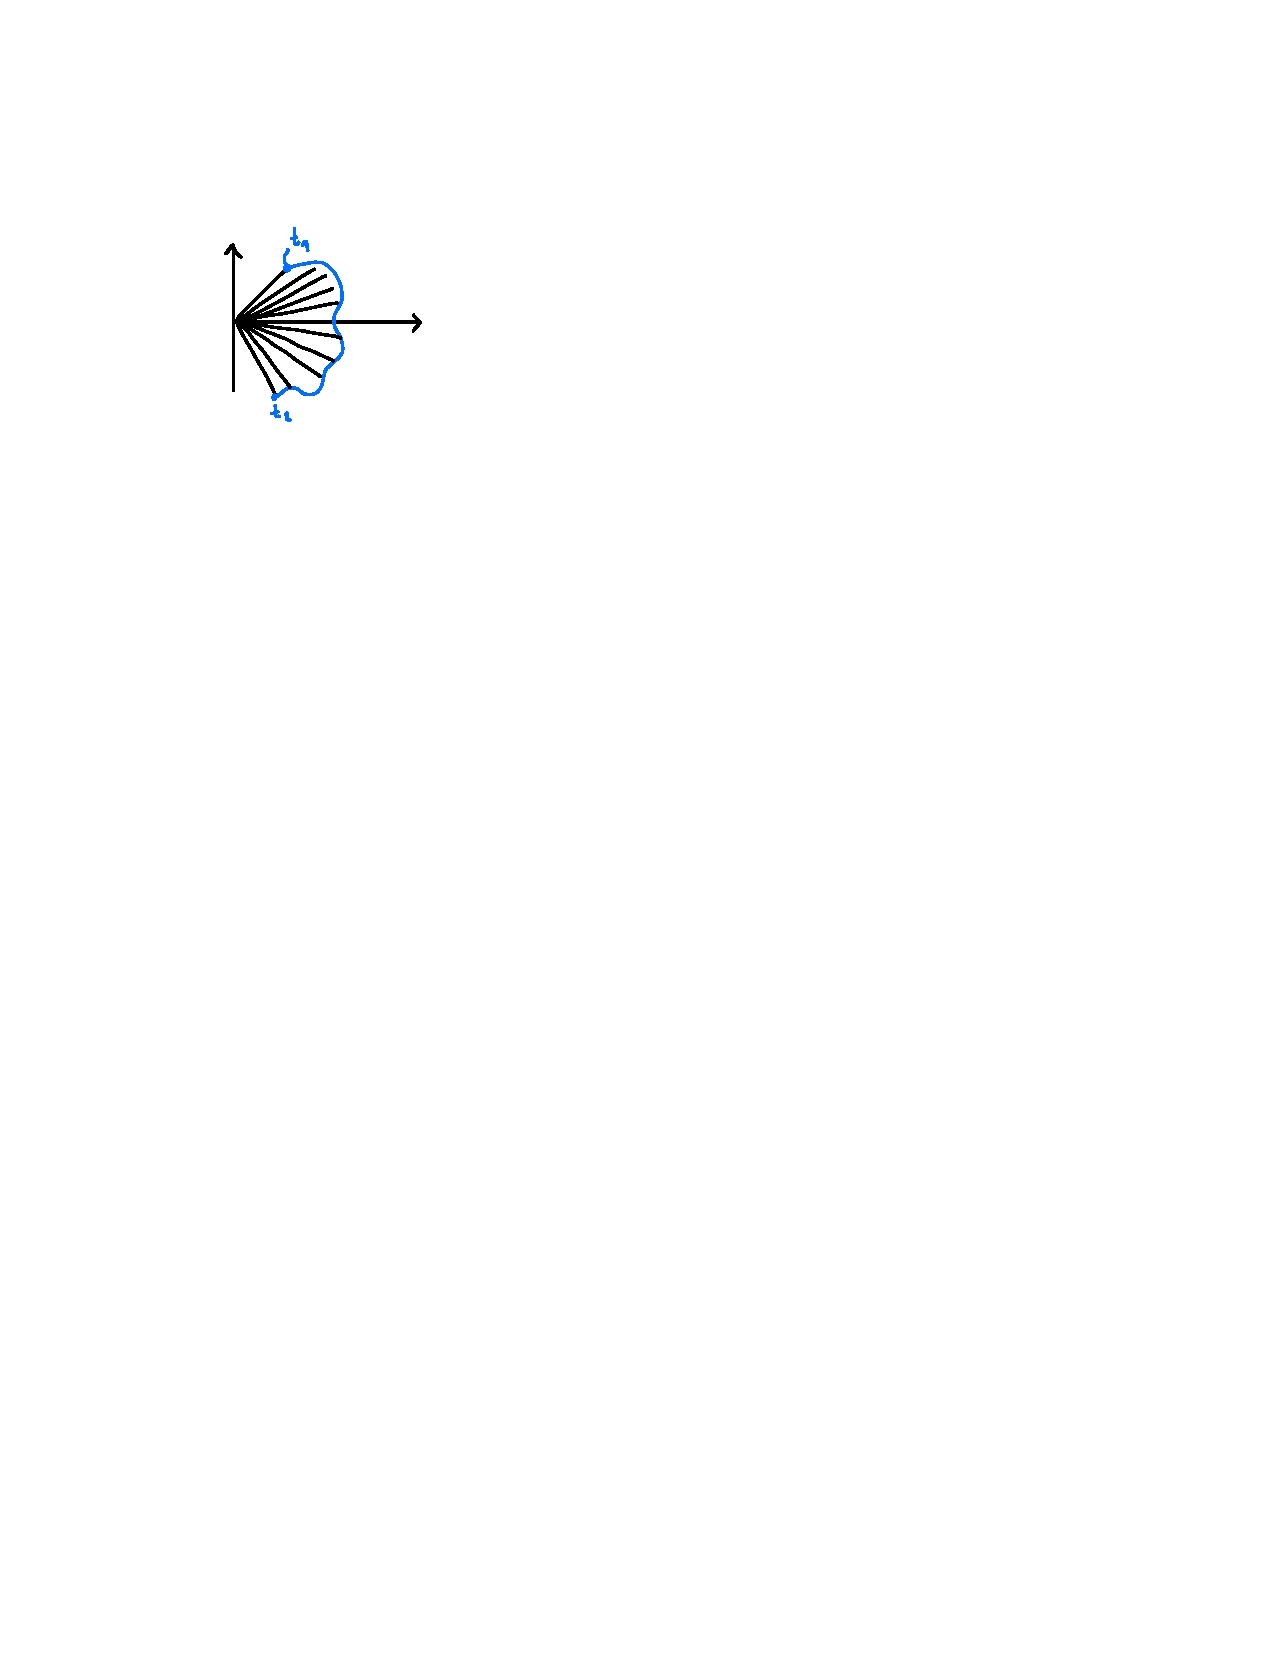
\includegraphics[width=0.6\linewidth]{src/Integralrechnung/sektor.pdf}
    \end{minipage}
    \begin{minipage}{0.65\linewidth}
        \begin{itemize}
            \item Polarkoordinaten
            \item[] $ \displaystyle A= \frac{1}{2} \int_{\varphi_1}^{\varphi_2} \rho^2(\varphi) \, d\varphi $
        \end{itemize}
    \end{minipage}
    \begin{minipage}{0.34\linewidth}
        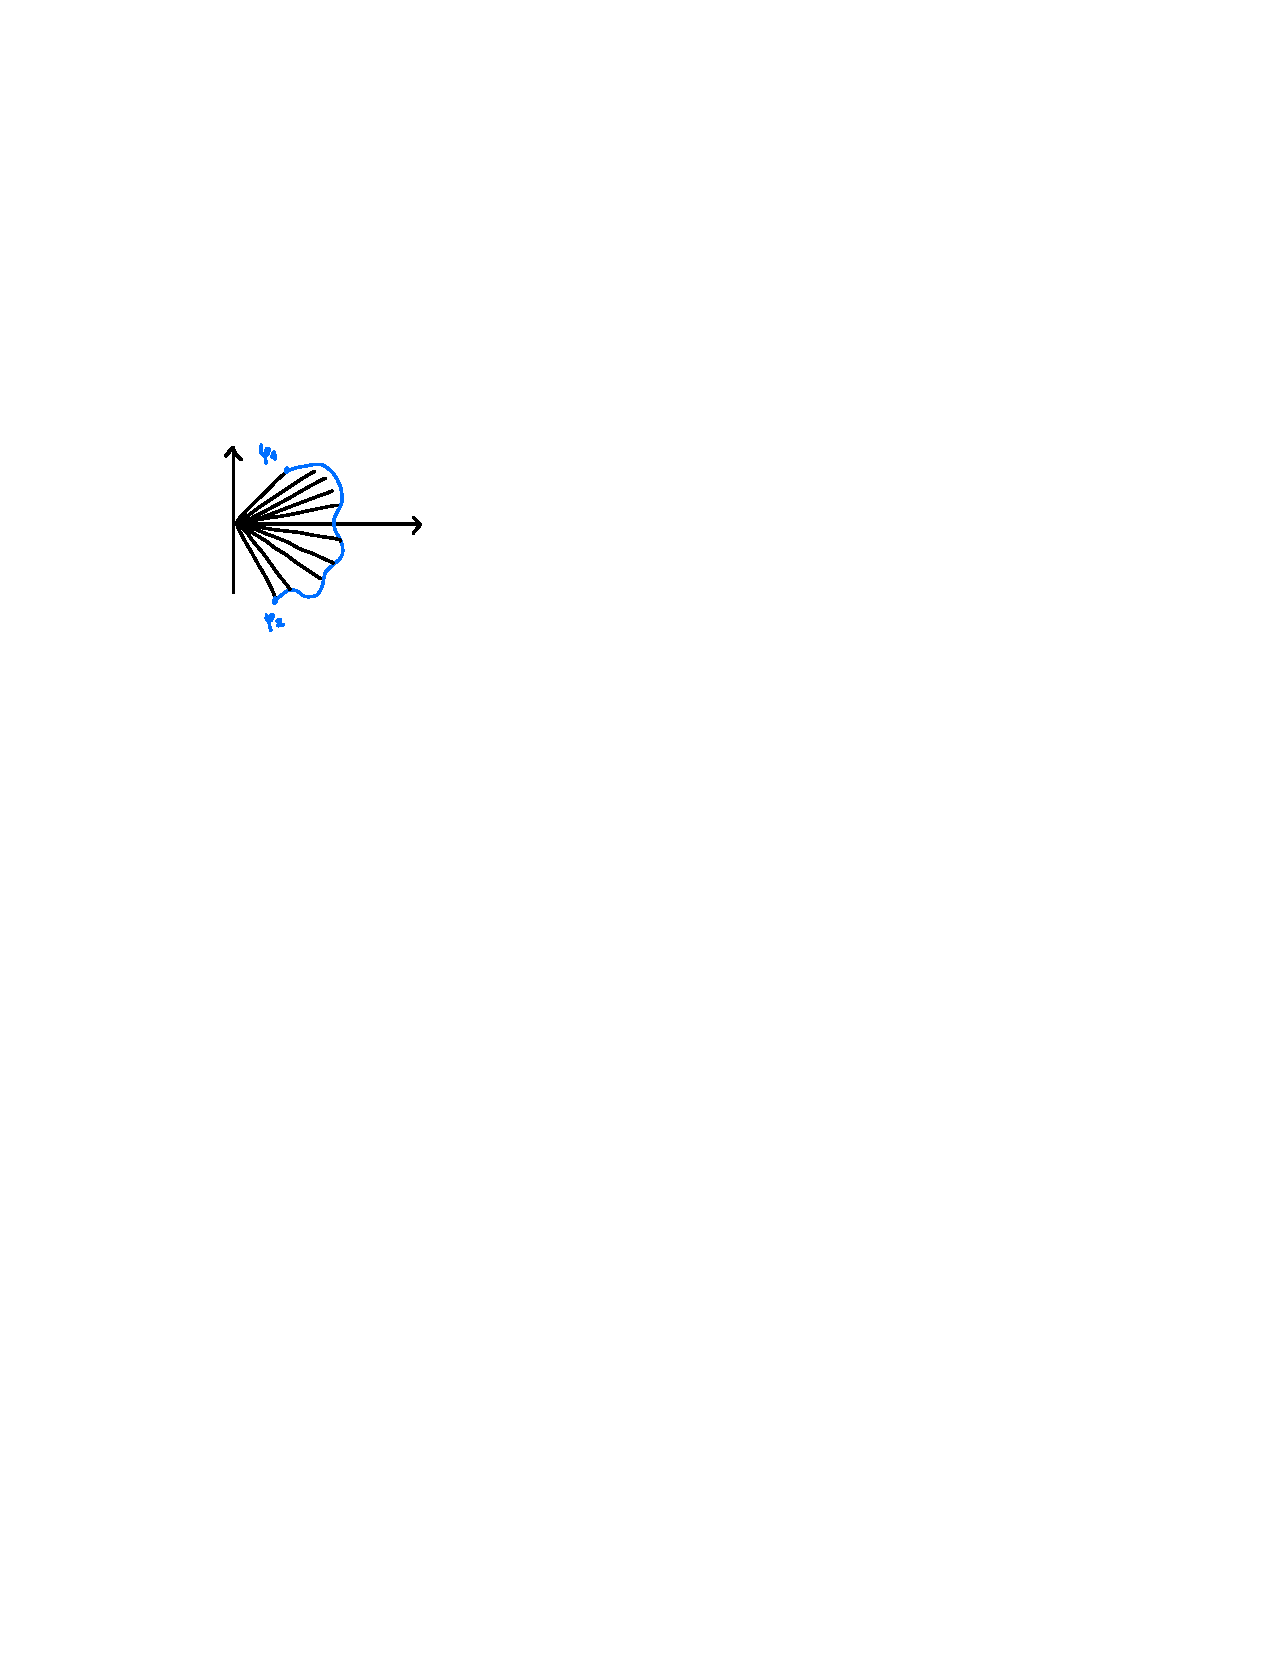
\includegraphics[width=0.6\linewidth]{src/Integralrechnung/polar.pdf}
    \end{minipage}

    
% \subsection{Flächenberechnungen}
%     \begin{minipage}{0.49\linewidth}
%         \begin{itemize}
%             \item Parametrisierung  
%             \begin{center}
%                 $\rvec=(x(t),y(t))^T$
%             \end{center}

%             $$
%             A= \int_{t_1}^{t_2} y \dxt \, dt
%             $$
%             \item Sektorfläche
%             $$
%             A= \frac{1}{2} \int_{t_1}^{t_2} (x \dyt - y \dxt) \, dt 
%             $$
%             \item Polarkoordinaten
%             $$
%             A= \frac{1}{2} \int_{\varphi_1}^{\varphi_2} \rho^2(\varphi) \, d\varphi
%             $$
%         \end{itemize}
%     \end{minipage}
%     \begin{minipage}{0.38\linewidth}
%         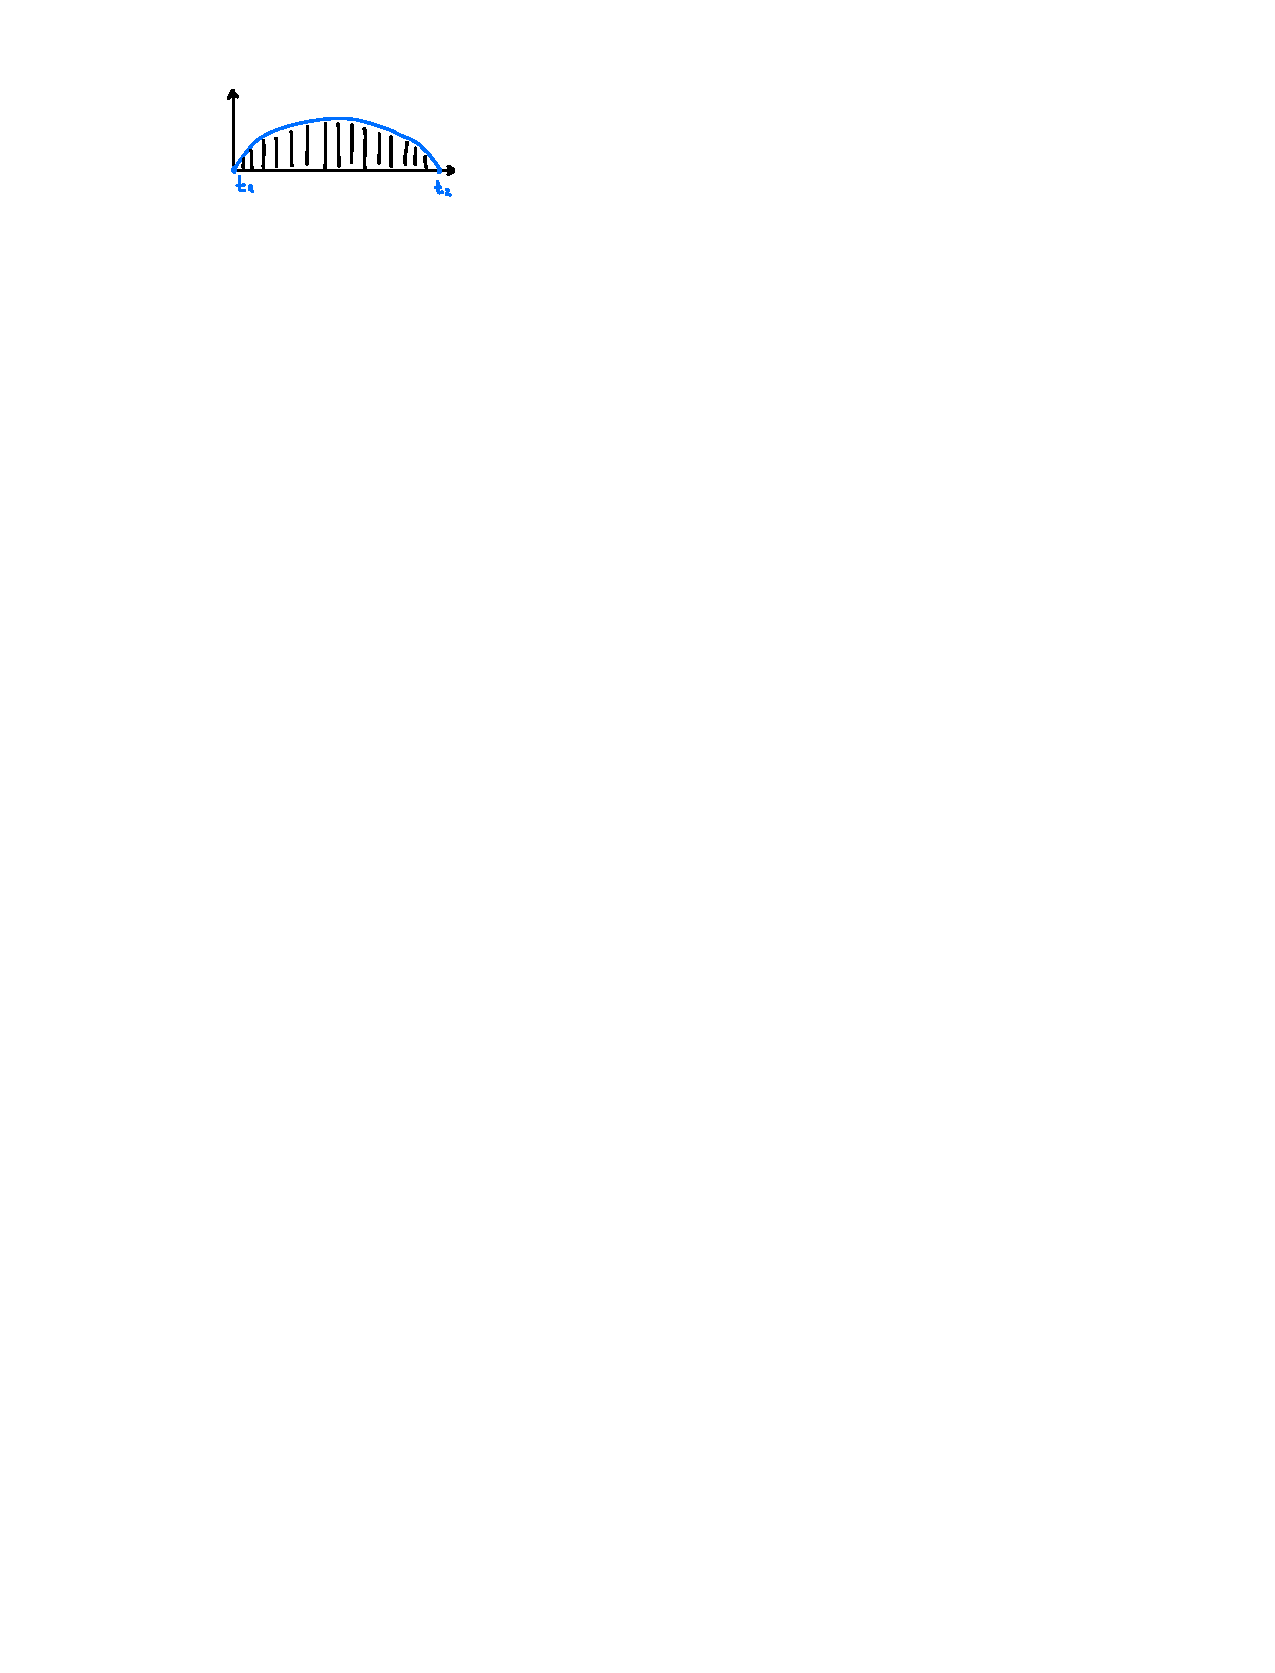
\includegraphics[width=\linewidth]{src/Integralrechnung/param.pdf}
%         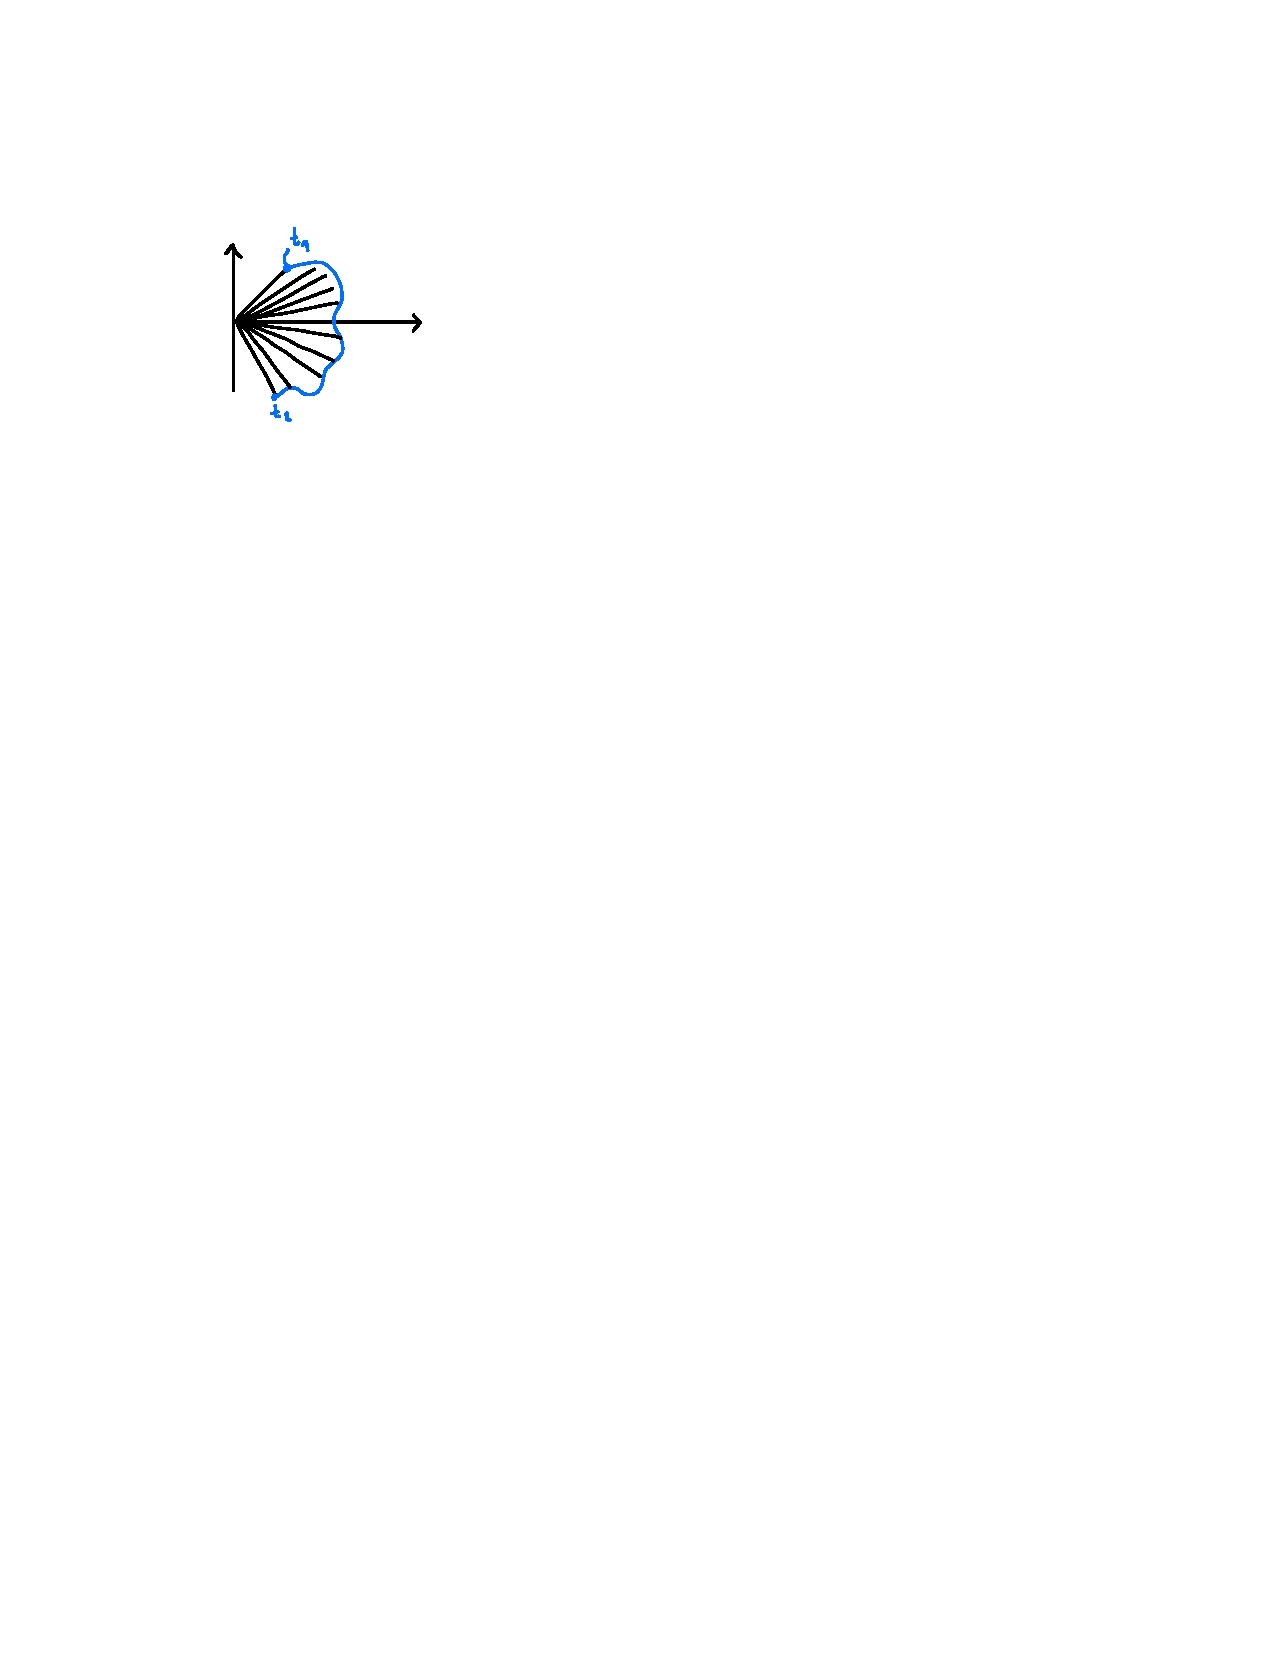
\includegraphics[width=\linewidth]{src/Integralrechnung/sektor.pdf}
%         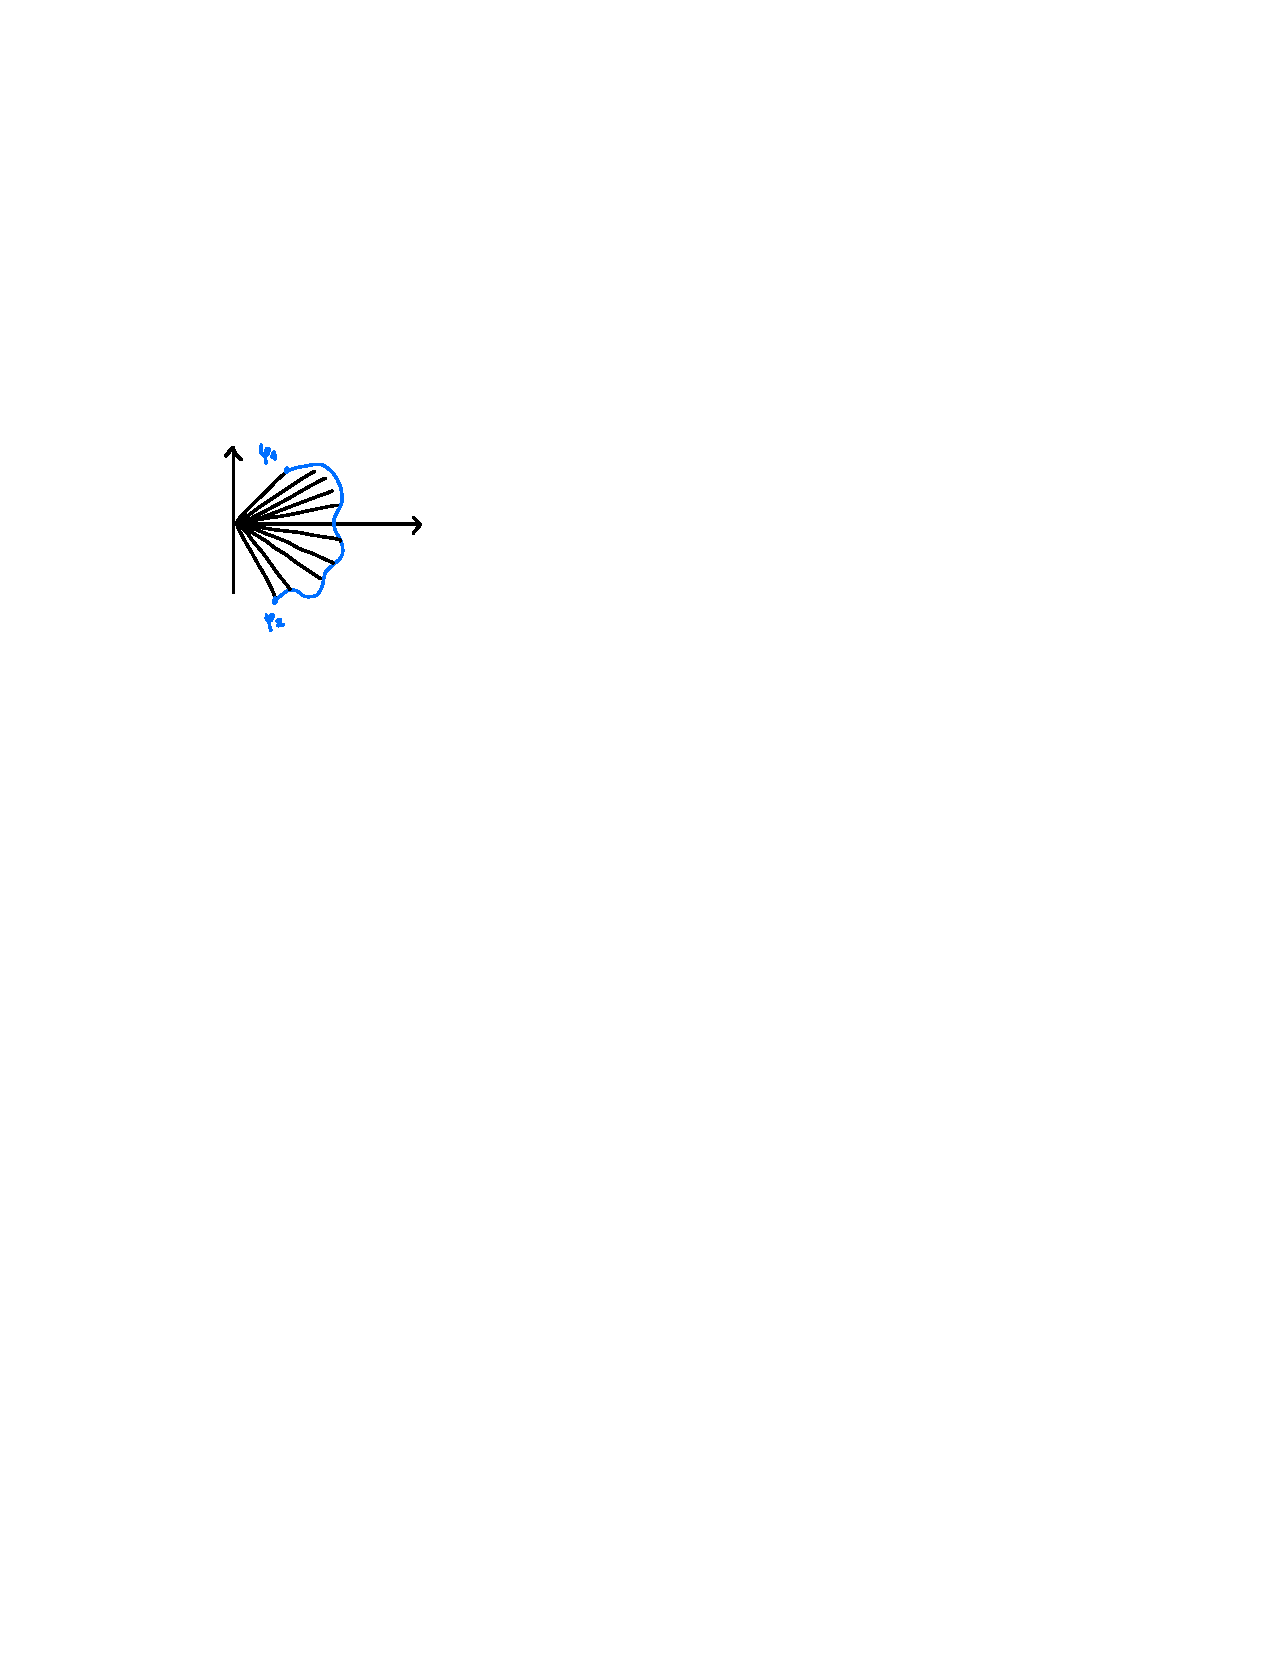
\includegraphics[width=\linewidth]{src/Integralrechnung/polar.pdf}
%     % \end{minipage}
    \cbreak
    \section{Mehrdimensionale Fkt. - Diff. Rechnung}
        % !TeX root = ../../ZF_bmicha_Ana.tex
\subsection{Fehlerrechnung \texorpdfstring{\hfill S.64}{S.64}}
    Die berechnete Grösse $f$ ist abhängig von den gemessenen Grössen $x,y$.
    Die gemessenen Grössen weichen mit den Messfehlern $dx,dy$ (auch $ \varDelta  x, \varDelta  y$ o.ä.) von der Realität ab.
    \begin{itemize}
        \item \textbf{Totales Differential / Absoluter Fehler}
            \mathbox{
                df \approx f_x\ dx + f_y\ dy
            }
        \item \textbf{Relativer Fehler}
            \mathbox{
                \frac{df}{f}
            }
    \end{itemize}
    \subsubsubsection{Bemerkungen}
        \vspace{0.5em}
        \begin{minipage}{0.54\linewidth}
            \centering \vspace{4pt}
            $1\%$ Genauigkeit
            $$
                \frac{dx}{x} = 1\% = \frac{1}{100}
            $$          
        \end{minipage}
        \begin{minipage}{0.45\linewidth}
            \centering
            Messfehler von $1^\circ$
            $$
                d\alpha = \frac{\pi}{180}
            $$
        \end{minipage}
        \vspace{3mm}\\
        \textit{Hinweis: in alle Formeln die Messwerte einsetzen, auch beim relativen Fehler. Auch wenn sie fehlerbehaftet sind.}
        % !TeX root = ../../ZF_bmicha_Ana.tex
\subsection{Niveaulinien / -flächen}
    \vspace{0.5em}
    \begin{minipage}{0.4\linewidth}
        \begin{center}
            \underline{\textbf{2D}}
        \end{center}
        $$
            f(x,y) = C , \quad C \in \mathbb{R}
        $$
        \begin{center}
            \textit{Höhenlinien}
        \end{center}
    \end{minipage}
    \hspace{0.05\linewidth}
    \begin{minipage}{0.5\linewidth}
        \begin{center}
            \underline{\textbf{3D}}
        \end{center}
        $$
            f(x,y,z) = C , \quad C \in \mathbb{R}
        $$
        \begin{center}
            \textit{Flächen mit konst. Temp.}
        \end{center}
    \end{minipage}
        % !TeX root = ../../ZF_bmicha_Ana.tex
\subsection{Gradient} 
    %\vspace{-0.75em}
    $$
        \grad(f(x,y,z)) = \begin{pmatrix}
            f_x \\ f_y \\ f_z
        \end{pmatrix}
    $$
    \begin{itemize}
        \item Steht senkrecht auf Niveauflächen/ -linien.
        \item Zeigt in Richtung des grössten Anstiegs der Funktionswerte.
    \end{itemize}
    \subsubsection{2D - \texorpdfstring{$f(x,y)$}{f(x,y)}}
        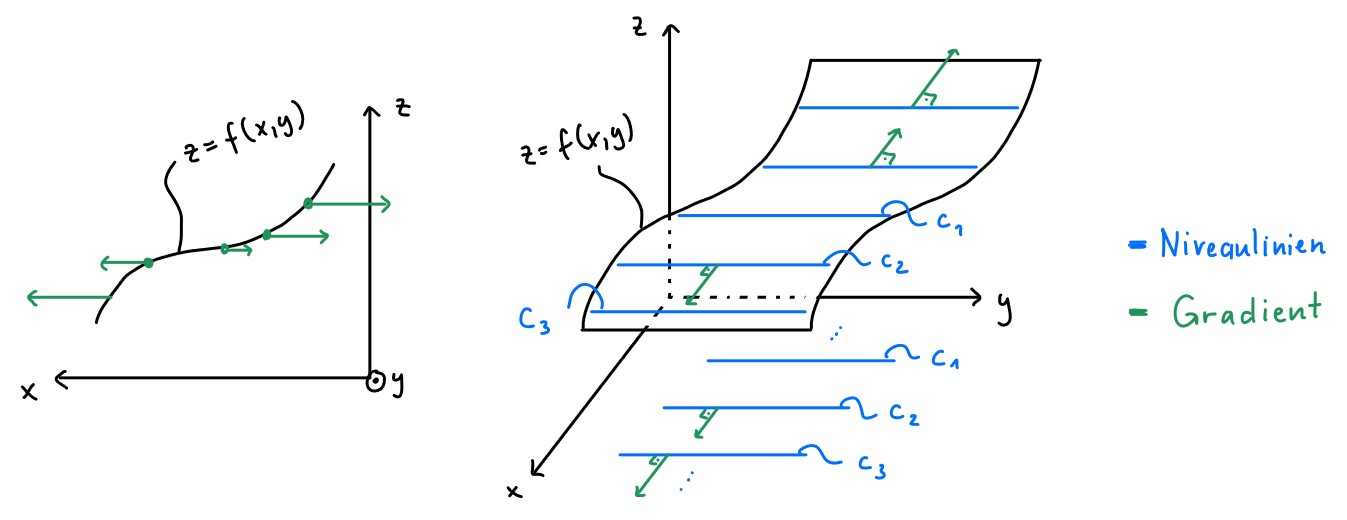
\includegraphics[width=\linewidth]{src/Mehrdimensionale-Funktionen_Differentialrechnung/Gradient 2D.jpg}
\cbreak 
    \subsubsection{3D - \texorpdfstring{$f(x,y,z)$}{f(x,y,z)}}
        \begin{center}
            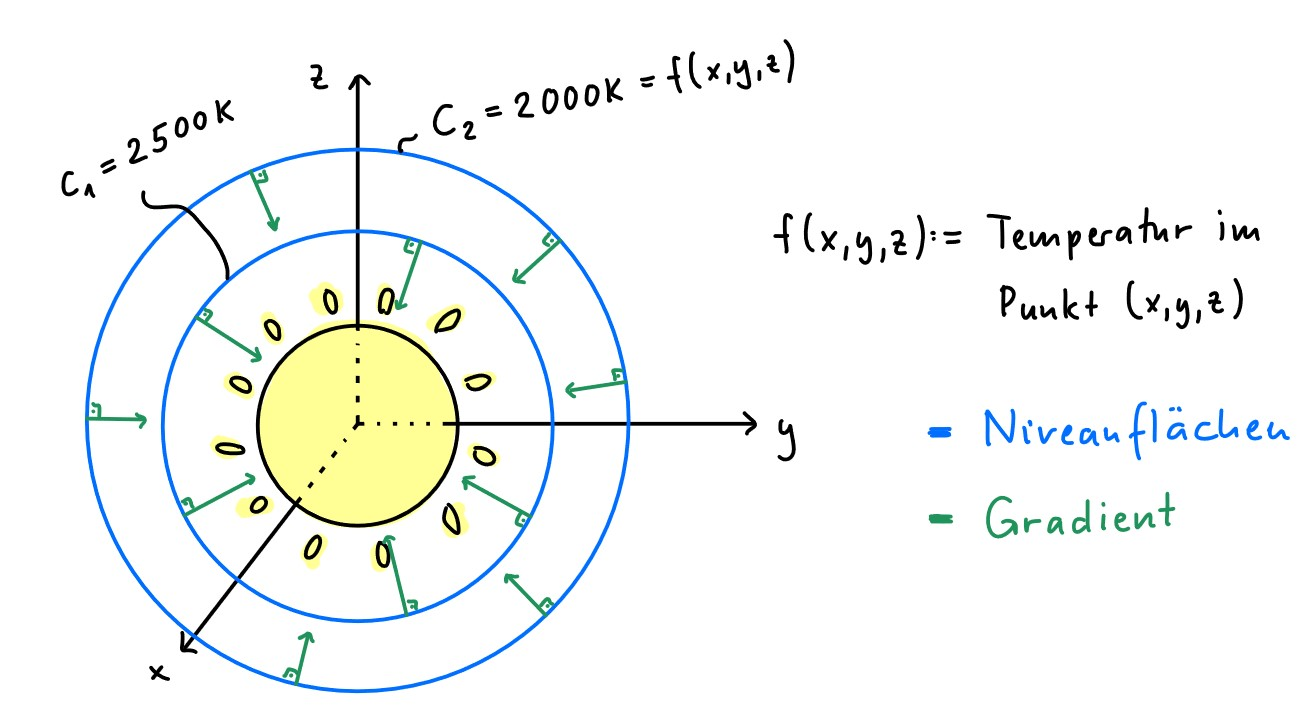
\includegraphics[width=0.8\linewidth]{src/Mehrdimensionale-Funktionen_Differentialrechnung/Gradient 3D.jpg}
        \end{center}
        
\vspace{3pt}
        % !TeX root = ../../ZF_bmicha_Ana.tex
\subsection{Tangentialebenen} \vspace{3pt}
    \subsubsection{Linearisierungsformel}
        \vspace{3pt}
        
        Tangentialebene an die Fläche: $z = f(x,y) $ im Punkt $P_o = (x_o, y_o, z_o)$ \\[5pt]  
        \textit{mit:}
        \mathbox{
            z = f(x_o,y_o) + f_x(x_o,y_o) (x\!-\!x_o) + f_y(x_o,y_o)(y\!-\!y_o)
        }
        \begin{enumerate}
            \item Wert für $f(x_o, y_o)$ finden
            \item $f_x$ bilden und $(x_o, y_o)$ einsetzen
            \item analog mit $f_y$ 
            \item Das ganze in der obigen Form zusammensetzen
        \end{enumerate}
        \vspace{5pt}
        
        \textit{mit:}
        \mathbox{
            0 = f_x(x_o,y_o,z_o)(x\!-\!x_o) + f_y(x_o,y_o,z_o)(y\!-\!y_o) + ...}
        \begin{enumerate}
            \item $f(x,y) \rightarrow \Tilde{f}(x,y,z)$  durch Subtraktion von z 
            \item $\Tilde{f}_x$ bilden und $(x_o, y_o, z_o)$ einsetzen
            \item analog für $\Tilde{f}_y$ und $\Tilde{f}_z$ wobei meist: $f_z = -1$
            \item Das ganze in der obigen Form zusammensetzen
        \end{enumerate}
        
          
        
    \subsubsection{Gradient} \label{sec:Gradient}
        \begin{itemize}
            \item $f(x,y,z) = C$ ist eine Niveaufläche
            \item $\grad(f)$ steht senkrecht auf Niveauflächen. ($\to \nvec$ )
            \item Gradient bilden und Koordinatenwerte des Punktes $P_o = (x_o,y_o,z_o)$ einsetzen.
            $$ \grad\left((f(x_o, y_o, z_o) \right) \!=\! \begin{pmatrix} f_x(x_o, y_o, z_o) \\ f_y(x_o, y_o, z_o) \\ f_z(x_o, y_o, z_o) \end{pmatrix} \! \Rightarrow \nvec \!= \!\begin{pmatrix} A \\ B \\ C \end{pmatrix}$$
            \item Ebene mit Normalenvektor $\nvec = (A,B,C)^T$:
            $$
                Ax + By + Cz = D
            $$
        \end{itemize}
        
        
    
        % !TeX root = ../../ZF_bmicha_Ana.tex
\subsection{Richtungsableitung}
    Steigung von $f$ in Richtung $\vec{e}$ im Punkt $\vec{r}_o$:
    $$
        D_{\vec{e}f} = \frac{\vec{e}}{ \lvert\vec{e}\,\rvert} \cdot \textrm{grad} f (\vec{r}_o)
    $$
        % !TeX root = ../../ZF_bmicha_Ana.tex
\subsection{Extremalstellen von \texorpdfstring{$f(x,y)$}{f(x,y)}}
    \vspace{0.25em}
    \begin{enumerate}
        \item Inneres untersuchen $\to$ $\textrm{grad}f \overset{!}{=} 0$
        \item Rand untersuchen
        \begin{itemize}
            \item Lagrange Multiplikatoren
            \begin{enumerate}
                \item $g(x,y)$ beschreibt Rand
                \item $\textrm{grad}f(x_o,y_o) = \lambda \cdot \textrm{grad}\, g(x_o,y_o)$\\[0.25em]
                      \phantom{llll}$\textrm{grad}\, g(x_o,y_o) \neq 0,\phantom{ll} \lambda \in \mathbb{R}$
                \item Gleichungssystem aus (a) und (b) lösen.
            \end{enumerate}
            \item Parametrisierung
            \begin{enumerate}
                \item Rand parametrisieren
                \item Parametrisierung in $f$ einsetzen
                \item Nach Parameter ableiten und nullsetzen.\\[0.25em] \phantom{llll}$f'(t) = 0$
            \end{enumerate}
        \end{itemize}
        \item Eckpunkte untersuchen
        \item Kandidaten vergleichen
    \end{enumerate}
    
\subsubsection{Verhalten an einer Extremalstelle} 

\begin{enumerate}
    \item Hesse-Matrix bilden: 
    $$ 
     H_f(x,y) = \begin{pmatrix} f_{xx} & f_{xy} \\ f_{yx} & f_{yy} \end{pmatrix}
    $$
    \item Die Koordinaten der ermittelten Extremalstelle einsetzen. Man erhält eine quadratische, symmetrische Matrix, da $f_{xy} \overset{!}{=} f_{xy}$. 
    \item Eigenwerte berechen: 
    $$
    \lambda_{1,2} = m \pm \sqrt{m^2 - p} 
    $$
    $ m = \frac{h_{11} + h_{22}}{2} \hspace{15pt} p = det(H) $
    \item Definitheit prüfen: 
    \begin{itemize}
        \item $\lambda_1, \lambda_2 > 0 \Rightarrow$ lokales Minimum
        \item $\lambda_1, \lambda_2 < 0 \Rightarrow $ lokales Maximum
        \item indefinit $\Rightarrow$ Sattelpunkt
        \item semidefinit $\Rightarrow$ keine Voraussage möglich
    \end{itemize}
\end{enumerate}
        \subsection{Satz von Schwarz}
    Satz: Die Reihenfolge von partiellen Ableitungen einer stetigen Funktion spielt keine Rolle.
    $$
        f_{xxyyzz} = f_{xzyxyz}
    $$
    \vspace{-1em}
        \subsection{Integrabilitätsbedingungen (IB)}\vspace{3pt}

    Geg.: $\phi(x,y), \psi(x,y)$\\[0.25em]
    Ges.: $f(x,y)$ mit:
    \begin{align*}
        f_x \equiv \phi \quad \textrm{und} \quad f_y \equiv \psi
    \end{align*}
    \begin{enumerate}
        \item IB prüfen (Satz von Schwarz):
            $$ \phi_y \equiv \psi_x$$
        \item $f(x,y)$ bestimmen (Konstante nicht vergessen!):
            $$ f = \int \phi\, dx = \int \psi\, dy $$
    \end{enumerate}
        % !TeX root = ../../ZF_bmicha_Ana.tex
\subsection{Verallgemeinerte Kettenregel}
    \vspace{-0.5em}
    $$
        Geg.: f(x,y,z),\quad x(t), y(t), z(\rho),\quad \rho(t)
    $$
    \vspace{0.25em}
    $$
        \frac{df}{dt} = \frac{\partial f}{\partial x}   \frac{dx}{dt} + \frac{\partial f}{\partial y} \frac{dy}{dt} + \frac{\partial f}{\partial z} \frac{dz}{d\rho} \frac{d\rho}{dt}
    $$
    \cbreak
    \section{Mehrdimensionale Fkt. - Int. Rechnung}
        % !TeX root = ../../ZF_bmicha_Ana.tex
\subsection{Flächen- \& Volumenintegrale}
    \vspace{0.5em}
    \begin{minipage}{0.4\linewidth}
        \begin{center}
            \underline{\textbf{2D}}
        \end{center}
        $$
            \iint f(x,y) \,\, dA
        $$
        \begin{center}
            \textit{Flächenintegral}
        \end{center}
    \end{minipage}
    \hspace{0.05\linewidth}
    \begin{minipage}{0.5\linewidth}
        \begin{center}
            \underline{\textbf{3D}}
        \end{center}
        $$
           \iiint f(x,y,z) \,\, dV
        $$
        \begin{center}
            \textit{Volumenintegral}
        \end{center}
    \end{minipage}
        % !TeX root = ../../ZF_bmicha_Ana.tex
\subsection{Dimensionsvergleich}
    \vspace{-1.25em}
    \begin{align*}
        \int f(x)\, dx &= Fl\ddot{a}che = \iint 1\, dA\\ % dirty hack is dirty
        \iint f(x,y)\, dA &= Volumen = \iiint 1\, dV\\
        \iiint f(x,y,z)\, dV &= ...
    \end{align*}
    \vspace{-0.75em}
        % !TeX root = ../../ZF_bmicha_Ana.tex
\subsection{Koordinatentransformationen \texorpdfstring{\hfill S.113}{S.113}}
    \begin{center}
        \textit{kartesisch:}
    \end{center}
    \begin{minipage}{0.49\linewidth}\vspace{-1em}
        \begin{align*}
            dA = dxdy \phantom{ml}
        \end{align*}
    \end{minipage}
    \begin{minipage}{0.49\linewidth}\vspace{-1em}
        \begin{align*}
            dV = dxdydz \phantom{ll}
        \end{align*}
    \end{minipage}

    \hrule
    \begin{center}
        \textit{zylindrisch:}
    \end{center}\vspace{-0.25em}
    \begin{minipage}{0.49\linewidth}\vspace{-1em}
        \begin{align*}
            x &= r \cos(\varphi)\\
            y &= r \sin(\varphi)\\\\[0.25em]
            dA &= r \, drd\varphi
        \end{align*}
    \end{minipage}
    \begin{minipage}{0.49\linewidth}\vspace{-1em}
        \begin{align*}
            x &= r \cos(\varphi)\\
            y &= r \sin(\varphi)\\
            z &= z\\[0.25em]
            dV &= r \, drd\varphi dz
        \end{align*}
    \end{minipage}\vspace{0.5em}

    \hrule
    \begin{center}
        \textit{sphärisch:}
    \end{center}\vspace{-0.25em}
    \begin{center}
        \begin{minipage}{0.49\linewidth}\vspace{-1em}
            \begin{align*}
                x &= r \sin(\theta)\cos(\varphi)\\
                y &= r \sin(\theta)\sin(\varphi)\\
                z &= r \cos(\theta)\\[0.25em]
                dV &= r^2 \sin(\theta) \, drd\varphi d\theta
            \end{align*}
        \end{minipage}
    \end{center}
        % !TeX root = ../../ZF_bmicha_Ana.tex
\subsubsection{Ellipsenkoordinaten}
    \begin{minipage}{0.49\linewidth}
        \vspace{0.5em}
        \underline{\textbf{Rand:}}\\
        \textit{implizit:}
        $$
            \left( \frac{x}{a} \right)^2 + \left( \frac{y}{b} \right)^2 = 1
        $$
        \textit{parametrisiert:}
        \begin{align*}
            x &= a \cdot \cos(\varphi)\\
            y &= b \cdot \sin(\varphi)\\
        \end{align*}
    \end{minipage}
    \begin{minipage}{0.5\linewidth}
        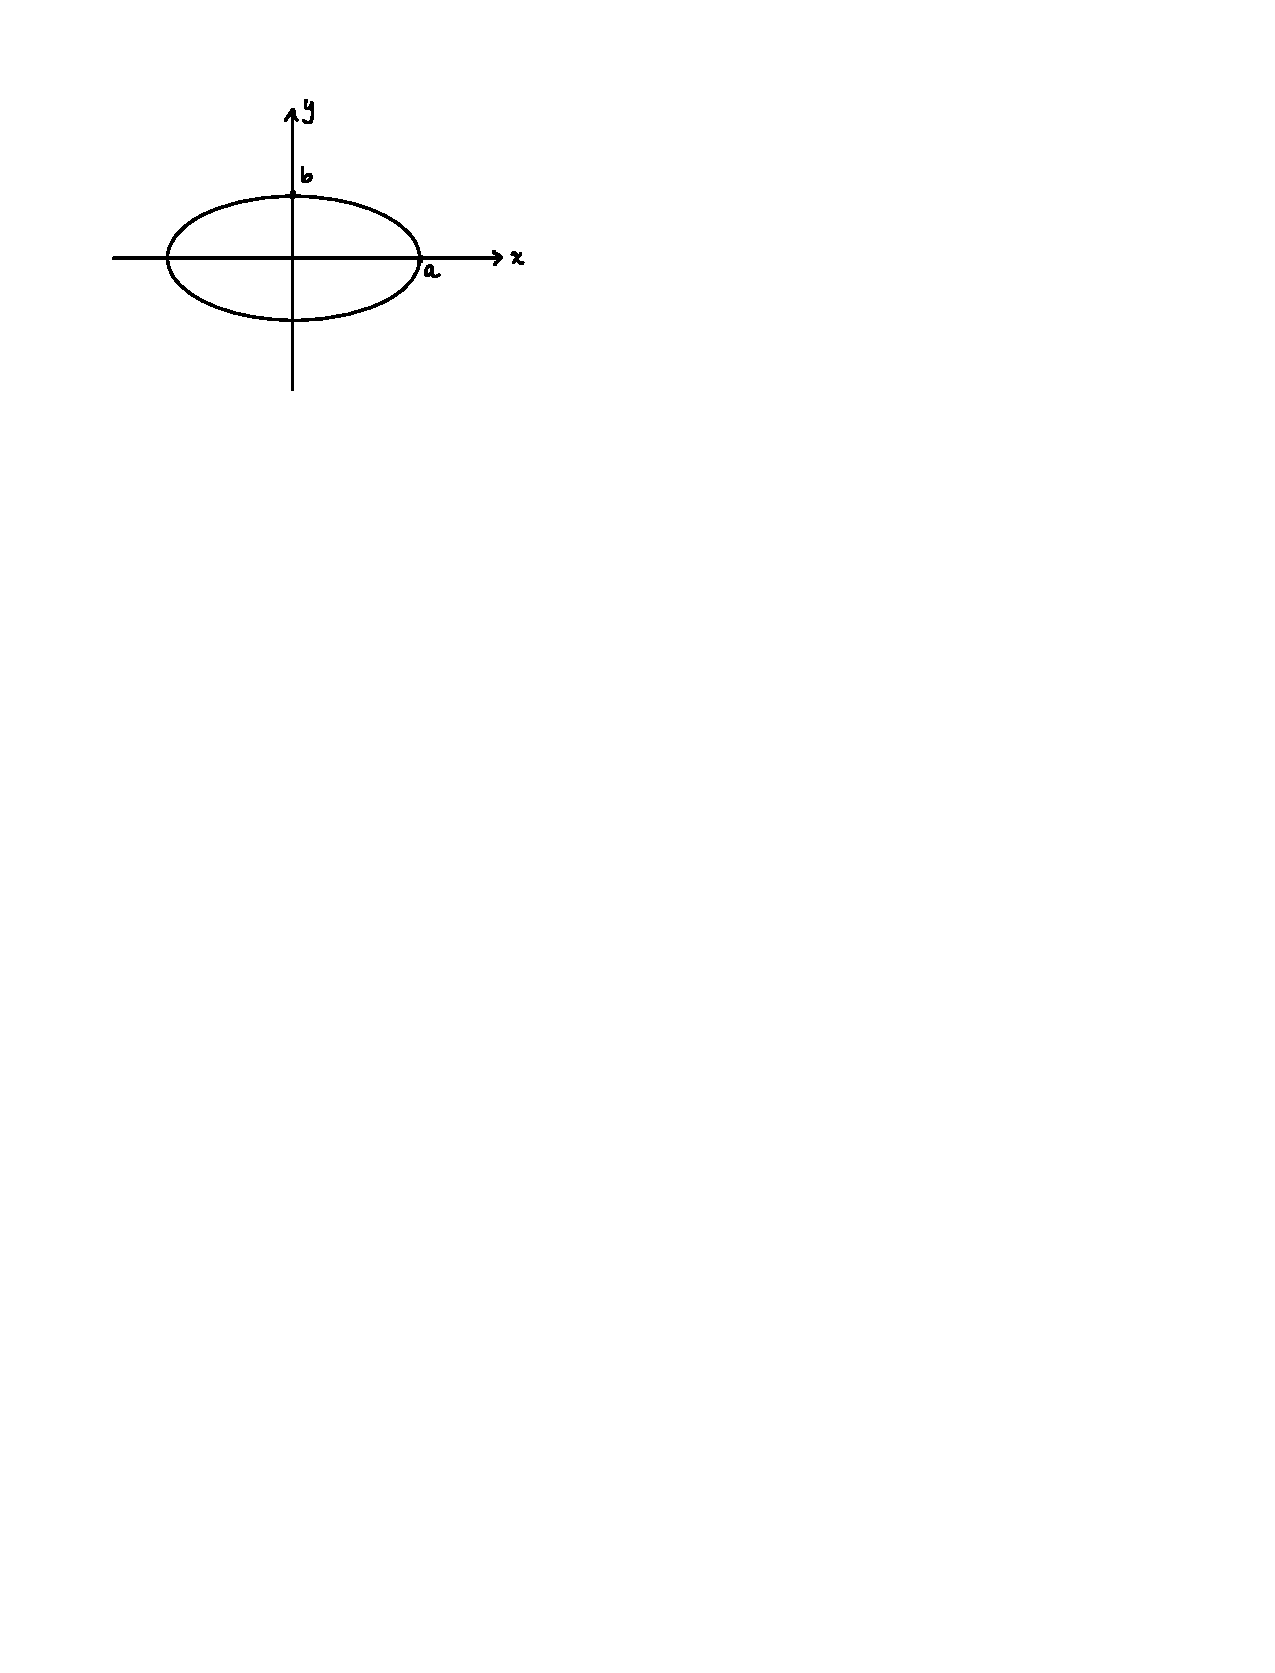
\includegraphics[width=\linewidth]{src/Mehrdimensionale-Funktionen_Integralrechnung/ellipse.pdf}
    \end{minipage}\vspace{-1em}
    \begin{minipage}{0.49\linewidth}
        \textbf{\underline{Fläche:}}
            \begin{align*}
                x &= a \cdot r \cdot \cos(\varphi)\\
                y &= b \cdot r \cdot \sin(\varphi)
            \end{align*}
    \end{minipage}
    \begin{minipage}{0.5\linewidth}
        \vskip4pt
        $dA = abr \, dr d\varphi$
        \vskip4pt
        mit $r \in \left[0, 1\right]$ und $\varphi \in \left[0, 2\pi\right]$
    \end{minipage}
        
        % !TeX root = ../../ZF_bmicha_Ana.tex
\subsubsection{Jacobi Matrix \& Determinante}
    Koordinatentransformation von $x,y,z$ nach $u,v,w$:
    $$
    x = x(u,v,w) \qquad y = y(u,v,w) \qquad z = z(u,v,w)
    $$
    $$
        \boldsymbol{J} = \begin{bmatrix}
            x_u & x_v & x_w\\
            y_u & y_v & y_w\\
            z_u & z_v & z_w
        \end{bmatrix}
    $$
    $$
        dx dy dz = \lvert \det(\boldsymbol{J}) \rvert \ du dv dw
    $$
    \cbreak
        % !TeX root = ../../ZF_bmicha_Ana.tex
\subsection{Schwerpunkte \texorpdfstring{\hfill S.76}{S.76}}\vspace{3pt}

    \subsubsection{2D}
    $\sigma(x,y)$: Flächendichte $[kg/m^2 ] $
        \begin{align*}
            &m = \iint \sigma(x,y) \, dA\\[0.25em]
            x_s =&\, \frac{1}{m} \iint x \cdot \sigma(x,y) \, dA\\
            y_s =&\, \frac{1}{m} \iint y \cdot \sigma(x,y) \, dA
        \end{align*}
    \textit{Keine Angabe für $\sigma$: $\sigma = 1$}
    \vspace{5pt}
    \subsubsubsection{Schwerpunkt eines Kreisausschnitts}
    \begin{minipage}{0.49\linewidth}
        \begin{align*}
        x_s &= 0 \\
        y_s &= \frac{2r^2 sin \alpha}{b} = r \frac{l}{b}
        \end{align*}
    \end{minipage}
    \begin{minipage}{0.49\linewidth}
        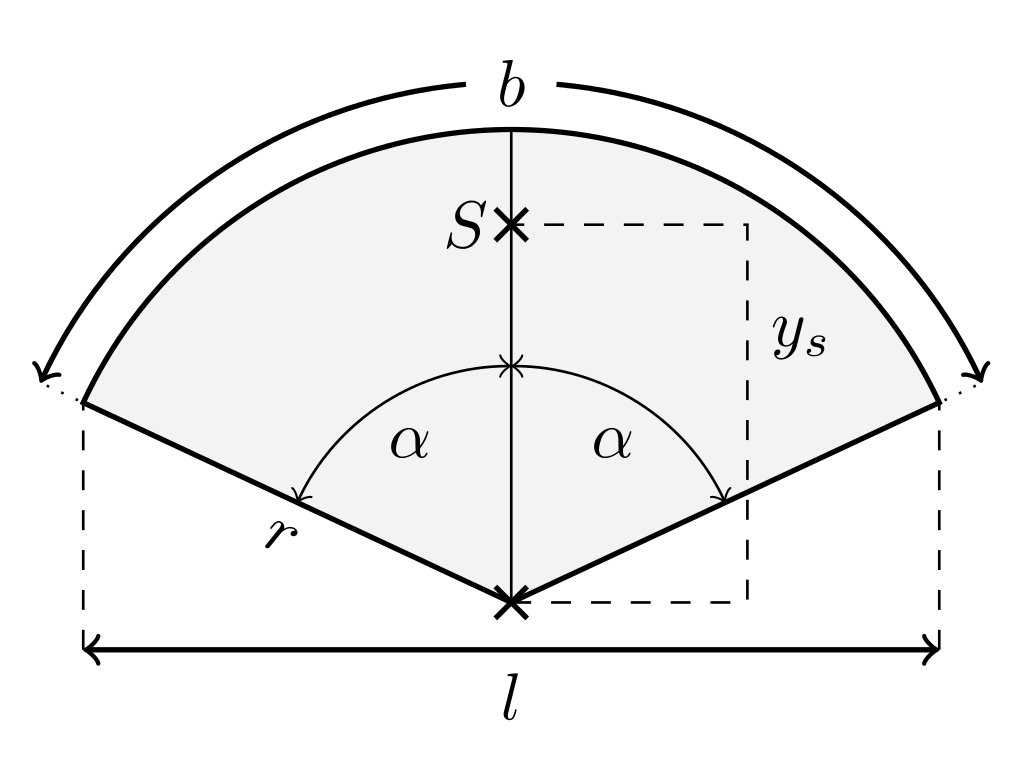
\includegraphics[width=0.95\linewidth]{src/Mehrdimensionale-Funktionen_Integralrechnung/1024px-Circular-sector-centroid.svg.png}
    \end{minipage}
    
    \subsubsubsection{Schwerpunkt eines Kreissegments}
    
    \begin{minipage}{0.49\linewidth}
        \begin{align*}
        x_s &= 0 \\
        y_s &= \frac{s^3}{12 A} - r\cdot \cos{\frac{\alpha}{2}}\\ 
        A &= \frac{r^2}{2} \cdot \left( \frac{\pi \cdot \alpha}{180}- \alpha \right)\\
        \left[  \alpha \right] &= \textrm{Grad}
        \end{align*}
    \end{minipage}
    \begin{minipage}{0.49\linewidth}
        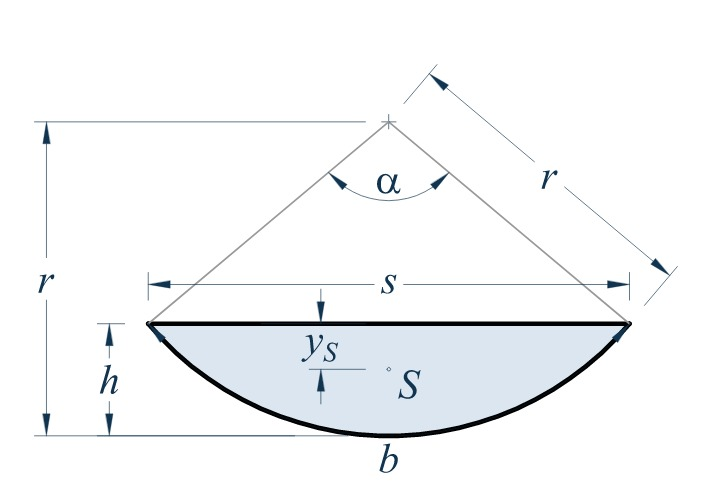
\includegraphics[width = \linewidth]{src/Mehrdimensionale-Funktionen_Integralrechnung/Kreissegment.jpeg}
    \end{minipage}
    
    \subsubsection{Zusammengesetzter Schwerpunkt}
    $$ x_s = \frac{1}{A_{ges}} \cdot \left( A_1 \cdot \Delta x_{s1} \pm A_2 \cdot \Delta x_{s2} \pm \dots \right) $$
    
    \subsubsection{3D}
    $\rho(x,y,z)$: Volumendichte $[kg/m^3 ] $
        \begin{align*}
            &m = \iiint \rho(x,y,z) \, dV\\[0.25em]
            x_s =&\, \frac{1}{m} \iiint x \cdot \rho(x,y,z) \, dV\\
            % y_s =&\, \frac{1}{m} \iiint y \cdot \rho(x,y,z) \, dV
            y_s =&\, \dots
        \end{align*}
        \vspace{-0.45em}
    \textit{Keine Angabe für $\rho$: $\rho = 1$}
    \vspace{0.5em}
    
    \cbreak
        

        
        % !TeX root = ../../ZF_bmicha_Ana.tex
\subsection{Trägheitsmoment \texorpdfstring{\hfill S.76}{S.76}}
    \subsubsection{2D}
        \textbf{Trägheitsmoment bzgl. einer Achse:}
        \begin{align*}
            I_x =& \iint_A \sigma(x,y) \cdot y^2 \, dA\\
            I_y =& \iint_A \sigma(x,y) \cdot x^2 \, dA
        \end{align*}
        \textbf{Trägheitsmoment eines Rotationskörper bzgl. seiner Achse:}
        \begin{align*}
         \textrm{explizit:} & \hspace{8pt} I_x =\frac{\pi}{2} \int y(x)^4  dx  \\
         \textrm{implizit:} & \hspace{8pt} I_x = \frac{\pi}{2} \int_{t_0}^{t_1} y(t)^4 \cdot |\dot{x}(t)| dt
         \end{align*}
        \textbf{Polares Trägheitsmom.} (bzgl. $z$-Achse/ Ursprung):
        \begin{align*}
            I_o = I_x + I_y = \iint_A \sigma(x,y) \cdot (x^2 + y^2) \, dA 
        \end{align*}
        \textit{Keine Angabe für $\sigma$: $\sigma = 1$}

    \subsubsection{3D}
        \textbf{Trägheitsmoment bzgl. Achse:}
        \begin{align*}
            I_x =& \iiint_V \rho(x,y,z) \cdot (y^2 + z^2) \, dV\\
            I_y =& \iiint_V \rho(x,y,z) \cdot (x^2 + z^2) \, dV \\
            I_z =& \iiint_V \rho(x,y,z) \cdot (x^2 + y^2) \, dV
        \end{align*}
        \textit{Keine Angabe für $\rho$: $\rho = 1$}
        \vskip5pt
    \small{Seien A bzw. B zwei disjunktive Körper (d.h. schneiden sich nicht) und a bzw. b ihr polares Trägheitsmoment um die z-Achse, so ist $I_{A \bigcup B} = a + b$ }
        
    \subsubsection{Satz von Steiner}
    \begin{minipage}{0.5\linewidth}
        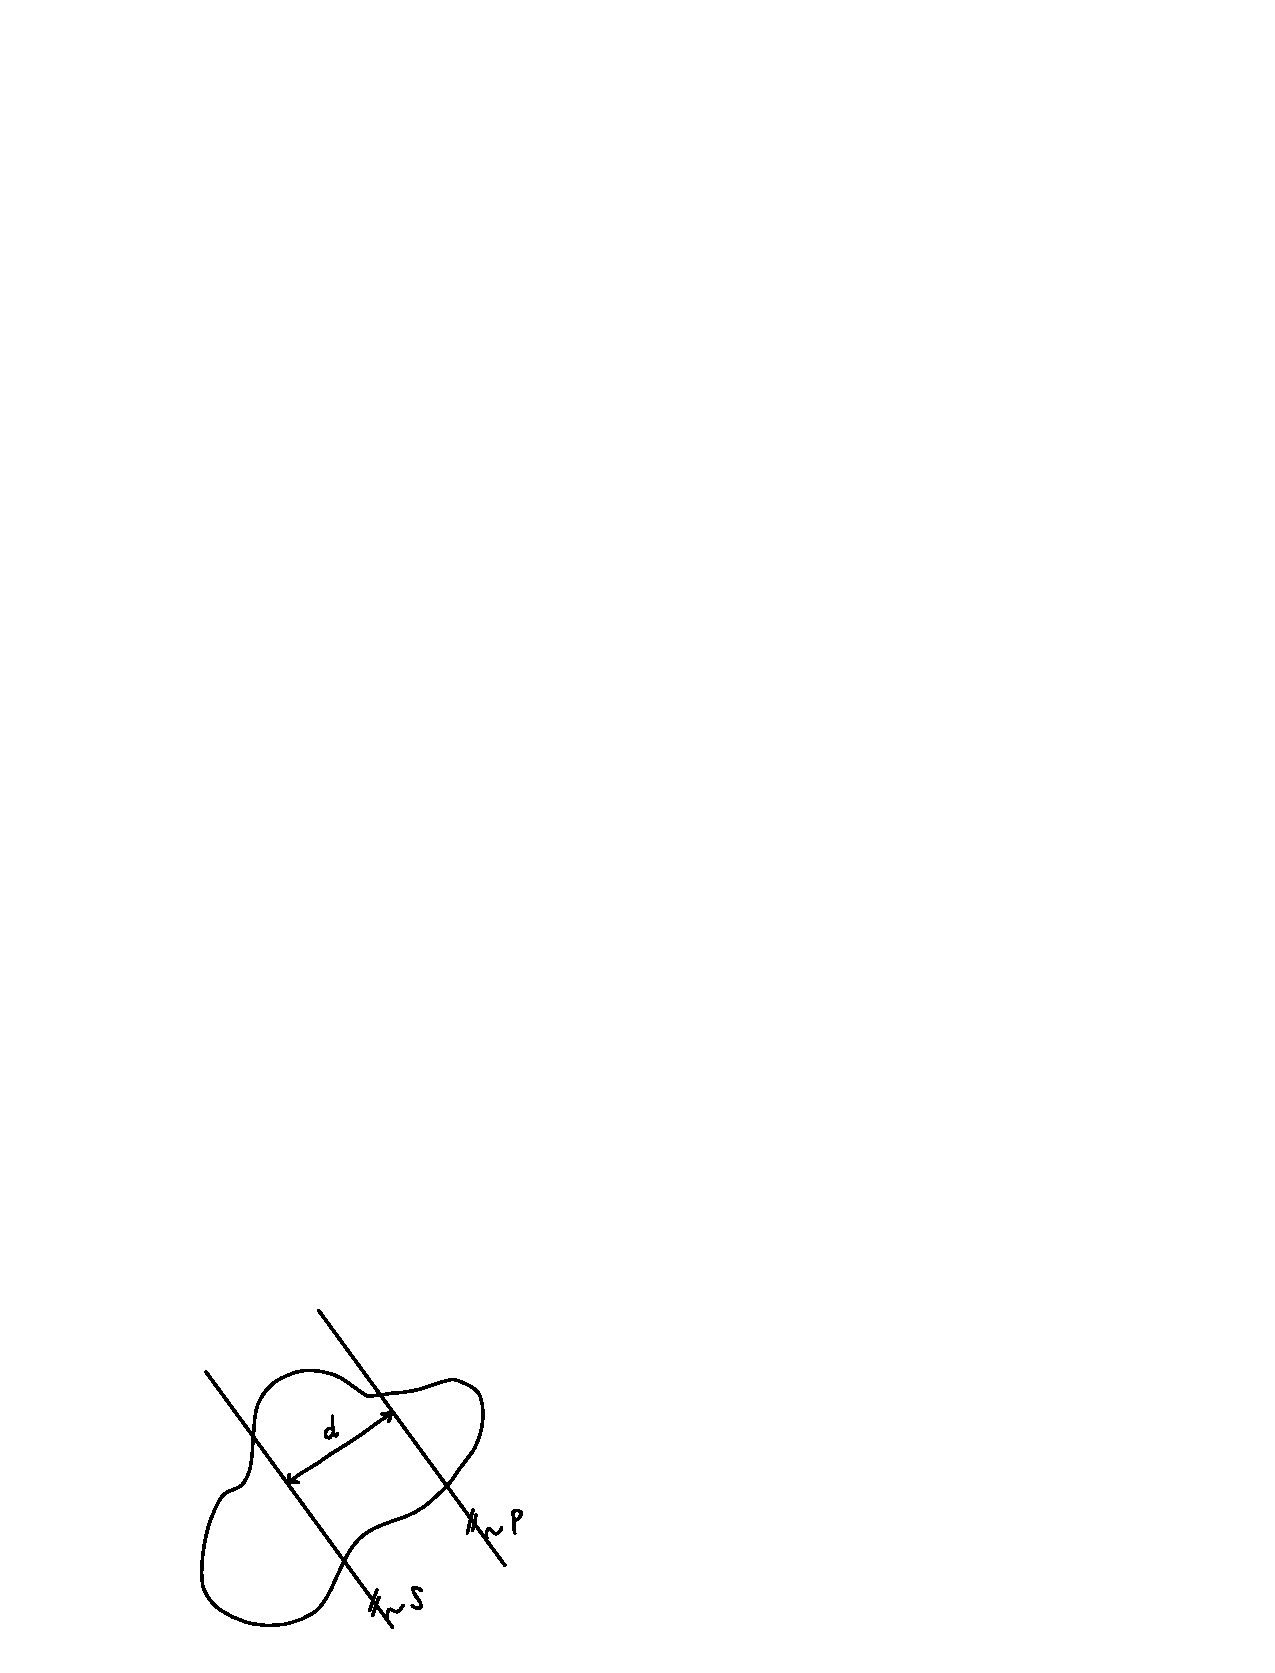
\includegraphics[width=\linewidth]{src/Mehrdimensionale-Funktionen_Integralrechnung/satz-von-steiner.pdf}
    \end{minipage}
    \hspace{0.05\linewidth}
    \begin{minipage}{0.4\linewidth}
        \begin{align*}
            I_p &=\,\, I_s + d^2 \cdot m\\
            m \vcentcolon&= Masse\\
            d \vcentcolon&= Abstand\\
        \end{align*}
    \end{minipage}
        % !TeX root = ../../ZF_bmicha_Ana.tex
\subsection{Leibnitz Theorem}
\vspace{-0.5em}
$$
    \frac{d}{dx} \left( \int_{a(x)}^{b(x)} f(x,t) dt \right) =
$$
$$
    \int_{a(x)}^{b(x)}  f_x(x,t) dt + f(x,b(x)) \, \frac{db(x)}{dx}  - f(x,a(x)) \, \frac{da(x)}{dx}
$$
\vspace{-0.5em}

        % !TeX root = ../../ZF_bmicha_Ana.tex
\subsection{Oberflächenintegrale}
    Spezialfall eines Flächenintegrals.\\    
    Flächeninhalt einer parametr. Oberfläche berechnen:
    \mathbox{
        \iint_{\mathcal{O}} d\mathcal{O} = \iint_{\mathcal{O}} \abs*{\vec{r}_u \times \vec{r}_v} du dv
    }
    \textbf{Parametrisierung der Oberfläche:}
    $$
        \vec{r} = \begin{pmatrix}
            x(u,v)\\
            y(u,v)\\
            z(u,v)
        \end{pmatrix}
    $$
    \begin{description}
        \item[Oberflächenelement:] $d\mathcal{O} = \abs*{\vec{r}_u \times \vec{r}_v} du dv$
        \item[Normalenvektor:]  $\vec{n} = \vec{r}_u \times \vec{r}_v$
        \item[Normaleneinheitsvektor:]  $\vec{n}_o = \frac{\vec{r}_u \times \vec{r}_v}{\abs*{\vec{r}_u \times \vec{r}_v}}$
    \end{description}
    {\small Oberflächenelement entspricht Jacobi-Determinante.} \vskip2mm
    \textit{Hinweis: ist die Fläche $F(x,y,z(x,y))$ gegeben, so lässt sich das Kreuzporudkt umgehen, wenn wir
    den Betrag des Gradienten nehmen. $\to$ \ref{sec:Gradient}} Achtung Korrketurfaktor! 
    \cbreak 
        \subsection{Rotationskörper \texorpdfstring{\hfill S.75}{S.75}}
Alle Funktionen müssen strikt monoton sein. 
\subsubsection{Rotation um x-Achse}
    \begin{minipage}{0.5\linewidth}
        \begin{align*}
            V_x &= \pi \int_a^b (f(x))^2 dx \\
            V_x &= \pi \left\lvert \int_{t1}^{t2} y^2 \dot{x} dt \right\lvert   
        \end{align*}
    \end{minipage}
\begin{minipage}{0.49\linewidth}
    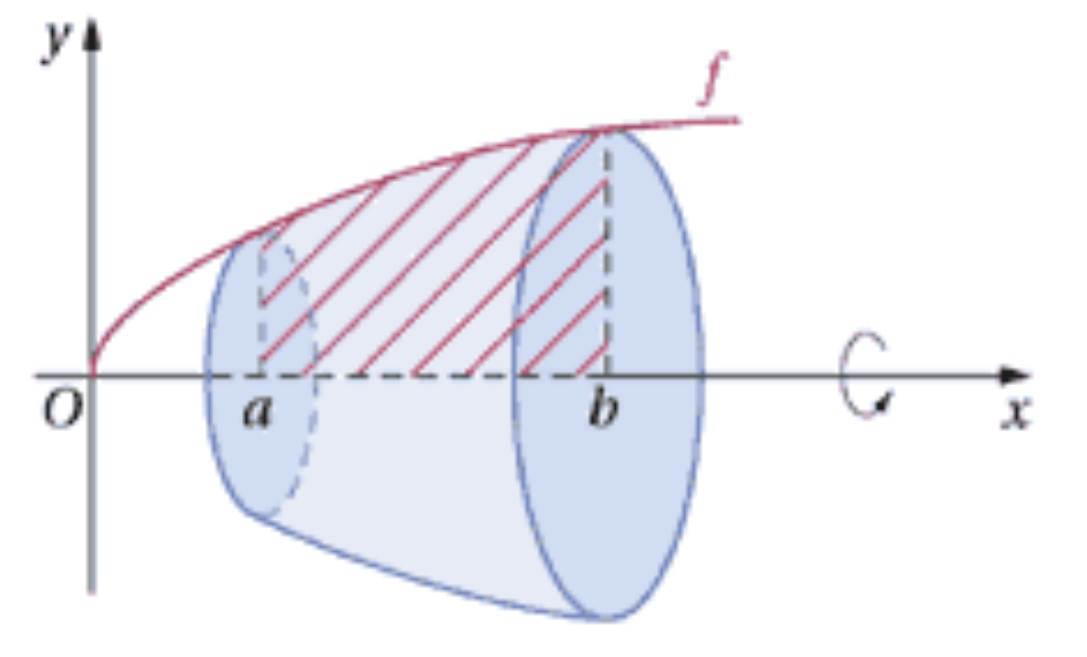
\includegraphics[width=\linewidth]{src/Mehrdimensionale-Funktionen_Integralrechnung/x_Achsen_Rotation.jpg}
\end{minipage}

\subsubsection{Rotation um y-Achse "disk integration"}
    \begin{minipage}{0.5\linewidth}
        \begin{align*}
             V_y &= \pi \int_a^b x^2 \cdot \left\lvert f'(x) \right\lvert dx \\
             V_y &= \pi \left\lvert \int_{t1}^{t2} x^2 \dot{y} dt  \right\lvert 
        \end{align*}
    \end{minipage}
    \begin{minipage}{0.49\linewidth}
         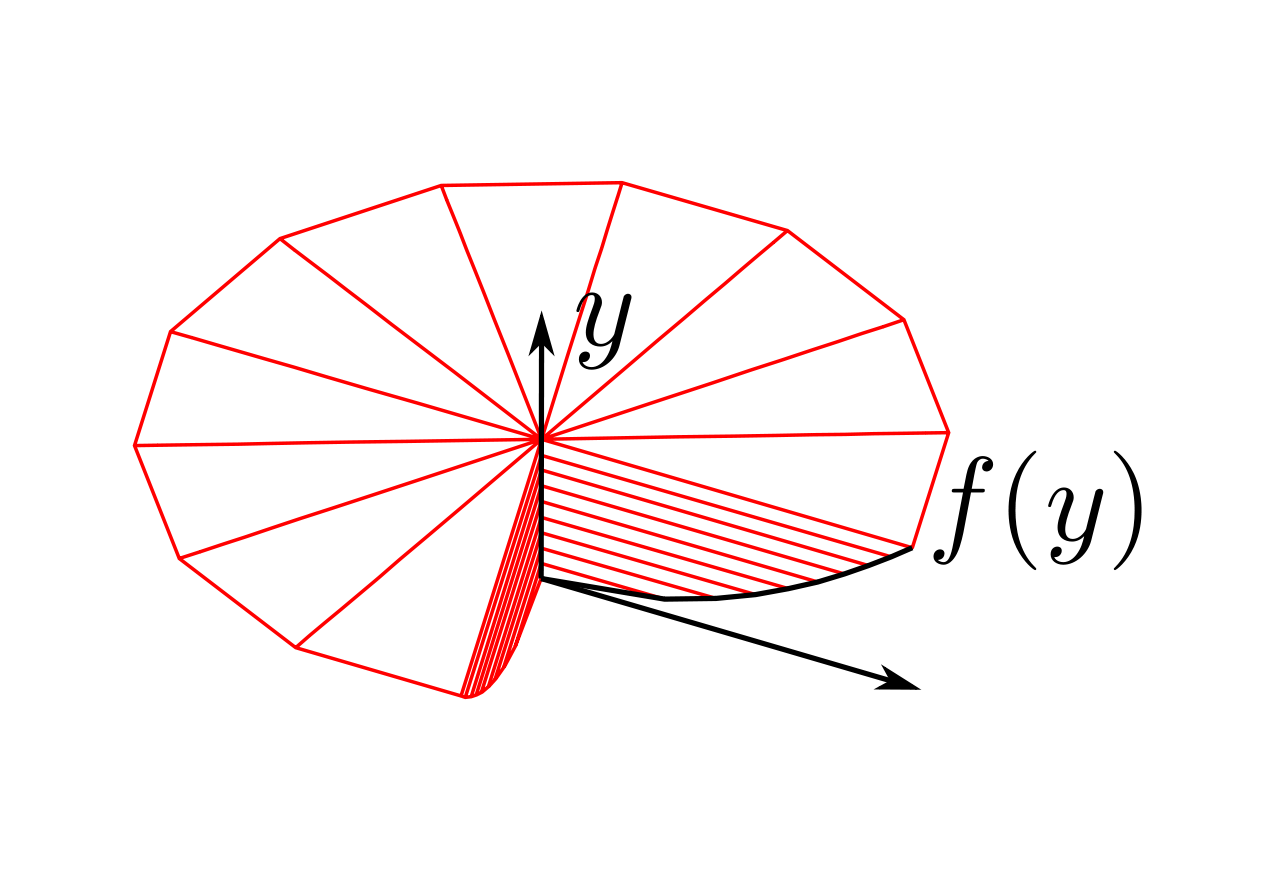
\includegraphics[width=\linewidth]{src/Mehrdimensionale-Funktionen_Integralrechnung/disk_integration.png}
    \end{minipage}

\subsubsection{Rotation um y-Achse "shell integration"}
    \begin{minipage}{0.5\linewidth}
        $$ V_y = 2\pi \int_a^b xf(x)dx $$
    \end{minipage}
    \begin{minipage}{0.49\linewidth}
         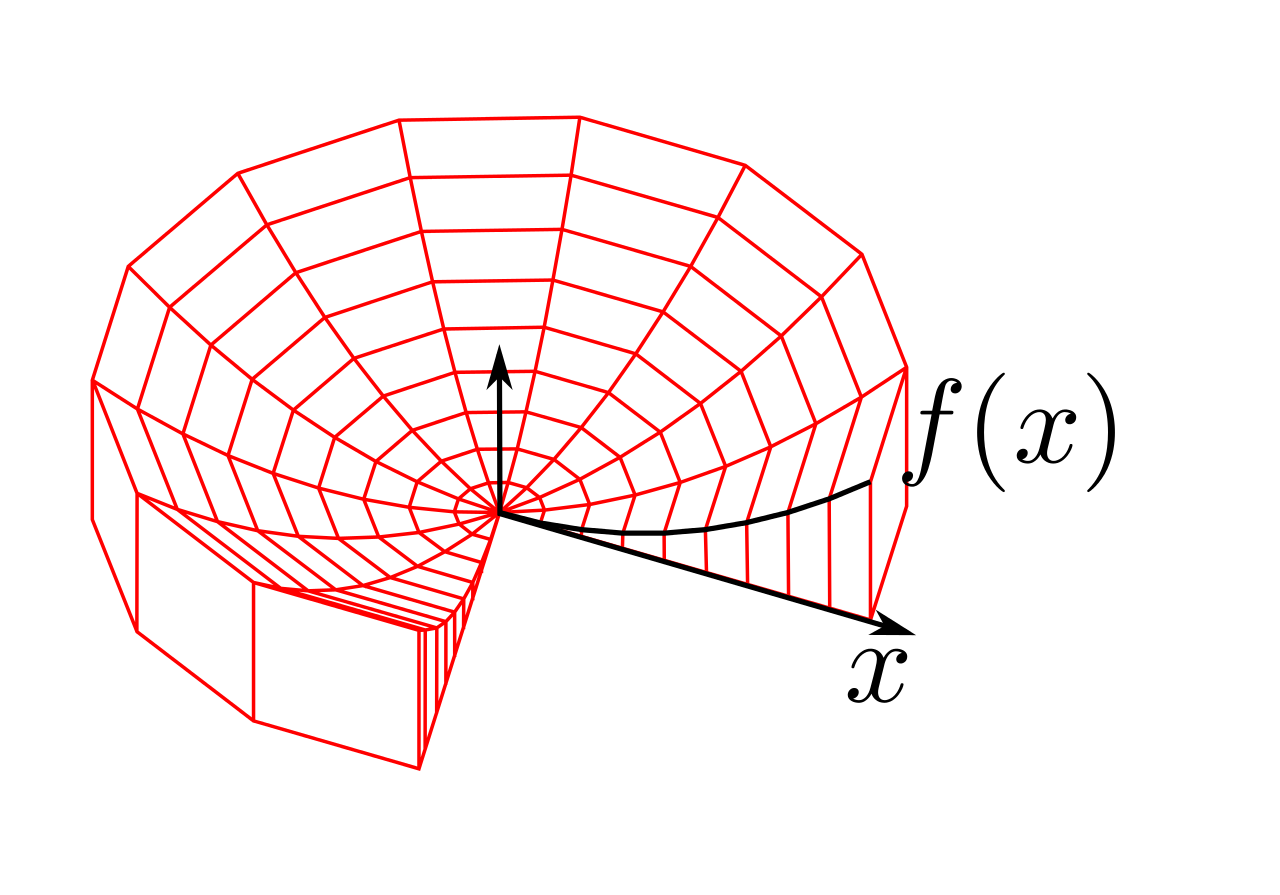
\includegraphics[width=\linewidth]{src/Mehrdimensionale-Funktionen_Integralrechnung/shell_integration.png}
    \end{minipage}



        % !TeX root = ../../ZF_bmicha_Ana.tex
\subsection{Flächenparametrisierungen}
Gängige Tricks falls die Fläche gegeben ist als:
    \begin{enumerate}
        \item $z = f(x,y)$
            $$
                \vec{r}(x,y) = \begin{pmatrix}
                    x\\y\\f(x,y)
                \end{pmatrix}
            $$
        \item $z = f(r,\varphi)$
            $$
                \vec{r}(r,\varphi) = \begin{pmatrix}
                    r\cos(\varphi)\\r\sin(\varphi)\\f(r,\varphi)
                \end{pmatrix}
            $$
        \item Rotationssymmetrische Fläche
            $$
                \vec{r}(t,\varphi) = \begin{bmatrix}
                    \mathrm{Rotations-}\\\mathrm{matrix}\\(\varphi)
                \end{bmatrix}
                \cdot
                \begin{pmatrix}
                    \mathrm{Param.}\\
                    \mathrm{Kurve}\\
                    \mathrm{(t)}
                \end{pmatrix}.
            $$
    \end{enumerate}
    \subsubsection{Rotationsmatrizen}
        \vspace{-1em}
        $$
        s_\varphi \vcentcolon= \sin(\varphi) \qquad c_\varphi \vcentcolon= \cos(\varphi)
        $$
        $$
        \begin{bmatrix}
            1 & 0 & 0\\
            0 & c_\varphi &-s_\varphi\\
            0 & s_\varphi & c_\varphi
        \end{bmatrix}_x
        \quad
        \begin{bmatrix}
            c_\varphi &0 & s_\varphi\\
            0 & 1 & 0\\
            -s_\varphi & 0 & c_\varphi
        \end{bmatrix}_y
        \quad\!
        \begin{bmatrix}
            c_\varphi &-s_\varphi& 0\\
            s_\varphi & c_\varphi& 0\\
            0 & 0 & 1
        \end{bmatrix}_z
        $$
    \cbreak
    \section{Vektoranalysis}
        % !TeX root = ../../ZF_bmicha_Ana.tex
Jedem Punkt im Raum $(x,y,z)$ wird ein Vektor zugeordnet.
% Bsp.: Geschwindigkeitsfeld eines Flusses - ''In welche Richtung fliesst das Wasser mit welcher Geschwindigkeit?''
$$
    \vec{v}(x,y,z) = \begin{pmatrix}
        u(x,y,z)\\v(x,y,z)\\w(x,y,z)
    \end{pmatrix}
$$
        % !TeX root = ../../ZF_bmicha_Ana.tex
\subsection{Allgemein} \vskip3pt
    \textbf{Gradient} \hfill $ f(x,y,z) \rightarrow \vec{v}(x,y,z)$
    $$
     \grad(f(u,v,w)) = \begin{pmatrix}
         f_u \\ f_v \\ f_w \end{pmatrix}
    $$
    \textbf{Divergenz} (Quellstärke) \hfill $\vec{v} \rightarrow f(x,y,z)$
        $$
            \mathrm{\div}(\vec{v}) = \nabla \cdot \vec{v} = u_x + v_y + w_z
        $$
    \textbf{Rotation} (Wirbelstärke) \hfill $\vec{v} \rightarrow \vec{w}$
        $$
            \mathrm{rot}(\vec{v}) = \nabla \times \vec{v} = 
            \begin{pmatrix}
                w_y - v_z\\ u_z - w_x\\v_x - u_y
            \end{pmatrix}
        $$
    \subsubsection{Identitäten}
        \vspace{-1em}
        \begin{align*}
            \div(\vvec) = 0 & \Longleftrightarrow \textrm{quellenfrei}\\
            \rot(\vvec) = 0 & \Longleftrightarrow\textrm{wirbelfrei} \\
            \div(\rot(\vvec)) = 0 & \\
            \rot(\grad(f)) = 0 & \\
        \end{align*} 
        $$\div(\grad(f)) = f_{xx} + f{yy} + f_{zz} = \Delta = \textrm{Laplace Operator}$$
        \vspace{-0.25em}
        % !TeX root = ../../ZF_bmicha_Ana.tex
\subsection{Fluss \texorpdfstring{\hfill $\Phi$}{Phi}}
    \vspace{-1em}
    \begin{align*}
        \Phi &= \iint_A \vvec \cdot \novec \ dA &\textrm{Allgemein}\\
        \Phi &= \iint_A \vvec(\rvec(u,v)) \cdot (\rvec_u \times \rvec_v) \ du dv &\textrm{Parametr.}\\
        \Phi &= \iiint_V \div(\vvec) \ dV &\textbf{Satz\ v. Gauss} \\[0.125em]
        \Phi &_{\textrm{nach aussen}} = - \Phi_{\textrm{nach innen}}
    \end{align*} \vskip1pt
    \textit{Hinweis: Richtung von $\novec$ beachten!}

    \subsubsection{Satz von Gauss}
        Falls $\vvec$ in ganz $B$ \textbf{definiert} und einmal \textbf{stetig differenzierbar} (\textit{regulär}) ist, gilt
        $$
            \iint_{\partial B} \vvec \cdot \novec \ dO = \iiint_B \div(\vvec) \ dV,
        $$
        wobei $\partial B$ die geschlossene Oberfläche des Volumens $B$ bezeichnet.
        Der Normaleneinheitsvektor $\novec$ auf $\partial B$ zeigt von innen nach aussen.
        % !TeX root = ../../ZF_bmicha_Ana.tex
\subsection{Arbeit \texorpdfstring{\hfill $W$}{W}}
    \vspace{-1em}
    \begin{align*}
        W &= \int_C \vvec \ d \vec{r} &\textrm{Allgemein}\\
        W &= \int_C \vvec(\rvec(t)) \cdot \dot{\rvec}(t) \ dt &\textrm{Parametr.}\\
        W &= \iint_{A} \rot(\vvec) \cdot \novec \ dA & \textrm{Satz von Stokes}\\[0.125em]
        W &= f\left(P_{\textrm{Ende}}\right) - f\left(P_{\textrm{Anfang}}\right) &\textrm{Potentialfeld} \\[0.125em]
        W &_{\textrm{Hinweg}} = - W_{\textrm{Rückweg}}& 
    \end{align*} \vskip1pt
    \textit{Hinweis: Richtung von $\novec$ beachten!}
    
\columnbreak

    \subsubsection{Arbeit Berechnen}
        \vspace{0.5em}
        \resizebox*{0.99\linewidth}{!}{
            \tikzset{every picture/.style={line width=0.75pt}} %set default line width to 0.75pt        
            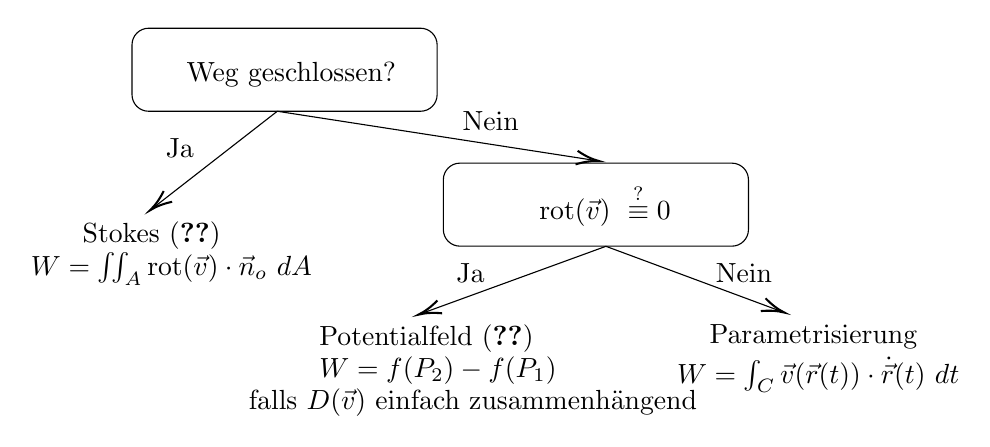
\begin{tikzpicture}[x=0.75pt,y=0.75pt,yscale=-1,xscale=1]
                \draw   (235,71) .. controls (235,66.58) and (238.58,63) .. (243,63) -- (374,63) .. controls (378.42,63) and (382,66.58) .. (382,71) -- (382,95) .. controls (382,99.42) and (378.42,103) .. (374,103) -- (243,103) .. controls (238.58,103) and (235,99.42) .. (235,95) -- cycle ;
                \draw   (385,136) .. controls (385,131.58) and (388.58,128) .. (393,128) -- (524,128) .. controls (528.42,128) and (532,131.58) .. (532,136) -- (532,160) .. controls (532,164.42) and (528.42,168) .. (524,168) -- (393,168) .. controls (388.58,168) and (385,164.42) .. (385,160) -- cycle ;
                \draw    (305,103) -- (245.25,149.5) ;
                \draw [shift={(243.67,150.73)}, rotate = 322.11] [color={rgb, 255:red, 0; green, 0; blue, 0 }  ][line width=0.75]    (10.93,-3.29) .. controls (6.95,-1.4) and (3.31,-0.3) .. (0,0) .. controls (3.31,0.3) and (6.95,1.4) .. (10.93,3.29)   ;
                \draw    (305,103) -- (458.02,126.69) ;
                \draw [shift={(460,127)}, rotate = 188.8] [color={rgb, 255:red, 0; green, 0; blue, 0 }  ][line width=0.75]    (10.93,-3.29) .. controls (6.95,-1.4) and (3.31,-0.3) .. (0,0) .. controls (3.31,0.3) and (6.95,1.4) .. (10.93,3.29)   ;
                \draw    (463.33,168.07) -- (374.88,200.31) ;
                \draw [shift={(373,201)}, rotate = 339.97] [color={rgb, 255:red, 0; green, 0; blue, 0 }  ][line width=0.75]    (10.93,-3.29) .. controls (6.95,-1.4) and (3.31,-0.3) .. (0,0) .. controls (3.31,0.3) and (6.95,1.4) .. (10.93,3.29)   ;
                \draw    (463.33,168.07) -- (547.46,199.3) ;
                \draw [shift={(549.33,200)}, rotate = 200.37] [color={rgb, 255:red, 0; green, 0; blue, 0 }  ][line width=0.75]    (10.93,-3.29) .. controls (6.95,-1.4) and (3.31,-0.3) .. (0,0) .. controls (3.31,0.3) and (6.95,1.4) .. (10.93,3.29)   ;

                % Text Node
                \draw (260,78) node [anchor=north west][inner sep=0.75pt]   [align=left] {Weg geschlossen?};
                % Text Node
                \draw (430,137) node [anchor=north west][inner sep=0.75pt]    {$\text{rot}(\vec{v}) \ \overset{?}{\equiv} 0$};
                % Text Node
                \draw (210,155) node [anchor=north west][inner sep=0.75pt]   [align=left] {Stokes (\ref{sec:SatzVonStokes})};
                % Text Node
                \draw (324,204.5) node [anchor=north west][inner sep=0.75pt]   [align=left] {Potentialfeld (\ref{sec:Potentialfeld})};
                % Text Node
                \draw (512,204.5) node [anchor=north west][inner sep=0.75pt]   [align=left] {Parametrisierung};
                % Text Node
                \draw (250,114.9) node [anchor=north west][inner sep=0.75pt]   [align=left] {Ja};
                % Text Node
                \draw (390,175) node [anchor=north west][inner sep=0.75pt]   [align=left] {Ja};
                % Text Node
                \draw (393,102) node [anchor=north west][inner sep=0.75pt]   [align=left] {Nein};
                % Text Node
                \draw (515,175) node [anchor=north west][inner sep=0.75pt]   [align=left] {Nein};
                % Text Node
                \draw (185,170) node [anchor=north west][inner sep=0.75pt]    {$W = \iint_{A} \rot(\vvec) \cdot \novec \ dA$};
                % Text Node
                \draw (324,220) node [anchor=north west][inner sep=0.75pt]    {$W = f(P_2) - f(P_1)$};
                \draw (290,235.5) node [anchor=north west][inner sep=0.75pt]    {falls $D(\vvec)$ einfach zusammenhängend};
                % Text Node
                \draw (496.33,220) node [anchor=north west][inner sep=0.75pt]    {$W = \int_C \vvec(\rvec(t)) \cdot \dot{\rvec}(t) \ dt$};
            \end{tikzpicture}
        }
\vspace{3pt}
    \subsubsection{Satz von Stokes} \label{sec:SatzVonStokes}
        Falls $\vvec$ auf ganz $A$ \textbf{definiert} und \textbf{stetig differenzierbar} (\textit{regulär}) ist, gilt
        $$
            \int_{\partial A} \vvec \ d \rvec = \iint_{A} \rot(\vvec) \cdot \novec \ dA,
        $$
        wobei $\partial A$ den geschlossenen Rand der Fläche $A$ bezeichnet.
        Der Normaleneinheitsvektor $\novec$ auf $A$ beschreibt mit der \textit{Rechte-Hand-Regel} den Umlaufsinn von $\partial A$.

    \subsubsection{Potentialfeld \texorpdfstring{$\vvec$}{v} zum Potential \texorpdfstring{$f$}{f}} \label{sec:Potentialfeld}
        Falls der Definitionsbereich $D(f)$ eines \textbf{wirbel\-freien} ($\rot(\vvec) \equiv 0$) Vektorfeldes \textbf{einfach zusammenhängend} (EZH) ist, nennen wir es \textit{konservativ}:
        \mathbox{
           D(f) \textrm{ EZH }\  \textit{und }\ \rot(\vvec) \equiv \vec{0} \quad \Rightarrow \quad \vvec = \grad(f).
        }
        $$ 
        \vvec = 
        \begin{pmatrix}
            u\\v\\w
        \end{pmatrix}
        =
        \begin{pmatrix}
            f_x\\f_y\\f_z
        \end{pmatrix}
        = \grad(f)
        $$ 

        $$
            f(x,y,z) = \int u \ dx = \int v \ dy = \int w \ dz
        $$
        Die Arbeit zwischen zwei Punkten entspricht der Potentialdifferenz.
        % \mathbox{
        %         $\vvec$ Potentialfeld &$\Longrightarrow$ $\rot(\vvec)=\vec{0}$
        % }
        \begin{empheq}[box=\fbox]{align*}
            \vvec \textrm{ Potentialfeld } &\Longrightarrow \rot(\vvec)=\vec{0}\\
            \vvec \textrm{ Potentialfeld } &\Longleftarrow \rot(\vvec)=\vec{0} \textrm{ \& } D(\vvec) = \textrm{ EZH}
        \end{empheq}
    
    
        % !TeX root = ../../ZF_bmicha_Ana.tex
\subsection{DGLs \& Vektorfelder}
    \vspace{0.5em}
    \mathbox[$\qquad \vvec = \begin{pmatrix} v_1\\v_2 \end{pmatrix}$]{
        y' = \frac{v_2}{v_1}
    }
    \subsubsection{Feldlinien \texorpdfstring{$y(x)$}{y(x)} \texorpdfstring{$\to$}{->} Vektorfeld \texorpdfstring{$\vvec$}{v}}
        \begin{enumerate}
            \item Feldliniengleichung nach $x$ ableiten $\to$ $y'(x)$
            \item Scharparameter eliminieren
            \item $\displaystyle y' = \frac{v_2}{v_1}$ $\to$ $\vvec = \begin{pmatrix} v_1\\v_2 \end{pmatrix}$
        \end{enumerate}
    \subsubsection{Vektorfeld \texorpdfstring{$\vvec$}{v} \texorpdfstring{$\to$}{->} Feldlinien \texorpdfstring{$y(x)$}{y(x)}}
        \vspace{0.5em}
        \begin{enumerate}
            \item $\displaystyle y' = \frac{v_2}{v_1}$
            \item DGL lösen
        \end{enumerate}
    \cbreak
    \section{Differentialgleichungen (DGL) \texorpdfstring{\hfill S.81}{S.81}}
        % !TeX root = ../../ZF_bmicha_Ana.tex
\subsection{Eigenschaften}
    \subsubsection{Existenz- \& Eindeutigkeitssatz}
        Sei $y' = f(x,y)$ in $D(f)$ \textbf{stetig} und \textbf{stetig partiell nach $\boldsymbol{y}$ differenzierbar}.
        \begin{itemize}
            \item[$\Rightarrow$] Für jeden Punkt $(x_o,y_o) \in D(f)$ gibt es \textit{genau eine} Lösung. 
            \item[$\Rightarrow$] Graphen von versch. Anfangswertproblemen (AWP) sind identisch oder disjunkt (kein gem. Pkt.).
        \end{itemize}
    \subsubsection{Linear}
        Eine DGL heisst \textit{linear}, falls alle $y$-Terme ($y, y', y'', \dots$) nur linear vorkommen.
        ($\to$ Kein: $sin(y')$, $y\cdot y'$, $e^y$, \dots)

% \textbf{Nützliche Integrale}
%     \begin{align*}
%         \int \frac{a}{ax + b} \ dx &= \ln(ax + b) + C, \quad C \in \mathbb{R}\\
%         \int \frac{\frac{1}{a}}{1 + \left(\frac{x}{a}\right)^2} \ dx &= \arctan\left(\frac{x}{a}\right) + C, \quad C \in \mathbb{R}
%     \end{align*}
% \textbf{Ordnung:}\\
%     Die Ordnung einer DGL entspricht dem Grad der höchsten Ableitung.
        % !TeX root = ../../ZF_bmicha_Ana.tex
\subsubsection{Separierbar} \label{sec:separierbareDGL}
    Separierbare DGLs können auf folgende Form gebracht werden:
    \mathbox{
        h(y(x)) \cdot y'(x) = g(x).
    }
    \begin{align*}
        h(y(x)) \cdot \frac{dy}{dx} &= g(x)\\
        \int h(y(x)) \cdot dy &= \int g(x) \cdot dx
    \end{align*}
        % !TeX root = ../../ZF_bmicha_Ana.tex
\subsubsubsection{Substitutionen}
    \begin{align*}
        u(x) &= \frac{y}{x}\\
        u(x) &= ax + by(x) + c\\
        u(x) &= y'(x)    
    \end{align*}
    Um $y'$ zu ersetzen, Substitution nach $y$ umformen und nach $x$ ableiten.
        % !TeX root = ../../ZF_bmicha_Ana.tex
\subsection{Orthogonaltrajektorien}
    \vspace{0.5em}
    \mathbox{
        y' = - \frac{1}{y_{OT}'}
    }
    \begin{enumerate}
        \item Kurvenschar $y(x)$ ableiten $\to y'(x)$
        \item Scharparameter eliminieren
        \item Obige Relation einsetzen und $y \to y_{OT}$
        \item DGL für $y_{OT}$ lösen
    \end{enumerate}
        % !TeX root = ../../ZF_bmicha_Ana.tex
\subsection{Enveloppe / Umhüllende} \label{sec:Enveloppe}
    \begin{empheq}[box=\fbox]{align*}
        F(x,y,C) &= 0\\
        \frac{\partial}{\partial C}F(x,y,C) &= 0
    \end{empheq}
    \begin{enumerate}
        \item Darstellung der Kurvenschar mit Scharparameter C finden: $F(x,y,C) = 0$
        \item Ausdruck für Scharparam. mit obigen Gleichungen bestimmen.
        \item Gefundenen Ausdruck $\widetilde{C}$ für Scharparam. in $F(x,y,C) = 0$ einsetzen $\to$ Enveloppengleichung
    \end{enumerate}
        % !TeX root = ../../ZF_bmicha_Ana.tex
\subsection{Lineare DGL 1. Ordnung}
    \vspace{0.5em}
    \mathbox%[$\quad q(x) \vcentcolon=$ Störfunktion]
    {
        y' + p(x) \cdot y = q(x)
    }
    $\triangleright$ $q(x) \vcentcolon=$ Störfunktion
    
    \subsubsection{Homogen}
        \vspace{0.5em}
        \mathbox{
            y' + p(x) \cdot y = 0
        }
        $\triangleright$ Immer separierbar. (\ref{sec:separierbareDGL})

    \subsubsection{Inhomogen}\label{sec:1.Ord-homogen}
        \vspace{0.5em}
        \mathbox{
            y' + p(x) \cdot y = q(x)
        }
        \begin{enumerate}
            \item $q(x) = 0$ setzen, homogene Lösung $y_h$ finden
            % $y_h' + p(x) \cdot y_h = 0$
            \item Partikuläre Lösung $y_p$ finden:
            \begin{itemize}
                \item Ansatz von Tabelle %(\ref{sec:linh-1orderTabelle})
                \item Lagrange-Methode %(\ref{sec:linh-1orderLagrange})
            \end{itemize}
        \end{enumerate}

    \subsubsubsection{Ansatz}
            \begin{enumerate}
                \item Ansatz für $y_p$ in inhomogene DGL einsetzen
                \item Koeffizientenvergleich
                \item $y = y_h + y_p$
            \end{enumerate}
            \begin{center}
                \renewcommand{\arraystretch}{1.25}
                \begin{tabular}{ll}
                    \hline
                    Störfunktion $q(x)$                                                                                                                       & Ansatz für $y_p(x)$                          \\ \hline\hline
                    Konstante                                                                                                                                 & $y_p = A$                                    \\
                    lineare Fkt.                                                                                                                              & $y_p = Ax + B$                               \\
                    Polynom Grad $n$                                                                                                                          & $y_p = Ax^n + Bx^{n-1} + \cdots$             \\
                    \begin{tabular}[c]{@{}l@{}}$A \sin(\omega x), A \cos( \omega x),$ \phantom{dirtl} \\ $A \sin(\omega x) + B \cos( \omega x)$\end{tabular} & $y_p = C \sin(\omega x) + D \cos( \omega x)$  \\
                    $A e^{{\color{blue}b}x}$                                                                                                                  & $y_p = B e^{{\color{blue}b}x}$               \\\hline
                \end{tabular}
            \end{center} 
                \vspace{0.5em}
                \textit{Falls der Ansatz nicht funktioniert:
                \begin{itemize}
                    \item Konstante Koeffizienten: mit $x$ multiplizieren
                    \item bei Euler-DGL: mit $ln(x)$ multiplizieren
                \end{itemize}
                }
                
        \subsubsubsection{Lagrange-Methode}
            
        %%
        %  \begin{enumerate}
        %        \item Lagrange-Ansatz $y_p$:\ $y_h = C \cdots \to y_p = C(x) \cdots$
        %        \item Ansatz in inhomogene DGL einsetzen
        %        \item Nach $C'(x)$ auflösen und integrieren
        %        \item $C(x)$ in $y_p$ einsetzen
        %        \item $y = y_p$
        %    \end{enumerate}
        %%
        
            \begin{enumerate}
                \item Ausgangsgleichung: $y' = f(X)y + g(x) $
                \item $y_h$ wie gewohnt berechnen ($g(x) := 0$)
                \item $y_p = y_h \cdot \int \frac{g(x)}{y_h}  \,dx $
                \item $y= y_h + y_p$
            \end{enumerate} 
        \vspace{1pt}
        
        % !TeX root = ../../ZF_bmicha_Ana.tex
\subsection{DGL Spezialfälle}
    \subsubsection{Clairaut'sche DGL}
        Entspricht Geraden mit Steigung $y'$ und Achsenabschnitten $g(y')$.
        \mathbox{
            y = y' \cdot x + g(y')
        }
        \begin{itemize}
            \item \textbf{Allgemeine Lösung:}
            $$
                y = C\cdot x + g(C)
            $$
            \item \textbf{Singuläre Lösung:}\\
                Enveloppe der allg. Lsg. bestimmen. (\ref{sec:Enveloppe})
        \end{itemize}

    \subsubsection{Exakte DGL}
        \vspace{0.5em}
        \mathbox{
            f_x + f_y \cdot y' = 0
        }
        \begin{itemize}
            \item Bedingung: $f_{xy} = f_{yx}$
            \item Allgemeine Lösung: $f(x,y) = C$
        \end{itemize}
    \cbreak
        % !TeX root = ../../ZF_bmicha_Ana.tex
\subsection{Lineare DGL n. Ordnung - konst. Koeff.}
    \subsubsection{Homogen}\label{sec:konst-koeff-homogen}
        \vspace{0.5em}
        \mathbox{
            a_n y^{(n)} + \cdots + a_2 y'' + a_1 y' + a_0 y = 0
        }
        \begin{enumerate}
            \item Ansatz \fbox{$y=e^{\lambda x}$} einsetzen $\to$ \textbf{char. Polynom}
            \item Nullstellen $\lambda_i$ des char. Polynom bestimmen
            \begin{itemize}
                \item $\lambda_1 \neq \lambda_2 \neq \cdots$, reell
                    $$
                        y = C_1 e^{\lambda_1 x} + C_2 e^{\lambda_2 x} + C_3 e^{\lambda_3 x}+ \cdots
                    $$
                \item $\lambda_1 = \lambda_2 = \cdots$, reell
                    $$
                        y = C_1 e^{\lambda_1 x} + C_2 {\color{magenta} x} e^{\lambda_2 x} + C_3 {\color{magenta} x^2} e^{\lambda_3 x} + \cdots
                    $$
                \item $\lambda_{1,2} = \lambda_{3,4} = \cdots = {\color{red}a} \pm i {\color{blue}b}$
                    \begin{align*}
                        y =\phantom{x} &e^{{\color{red}a}x} (C_1 \cos({\color{blue}b}x) + C_2 \sin({\color{blue}b}x)) +\\
                            {\color{magenta} x}&e^{{\color{red}a}x} (C_3 \cos({\color{blue}b}x) + C_4 \sin({\color{blue}b}x))+\\
                            {\color{magenta} x^2}&e^{{\color{red}a}x} (C_5 \cos({\color{blue}b}x) + C_6 \sin({\color{blue}b}x))+ \cdots
                    \end{align*}
            \end{itemize}
        \end{enumerate}
        \vspace{3pt}
        \small{\textit{Hinweis: damit das Verhalten der Lösungen für $x \to \infty$ beschränkt bleibt, müssen reelle Nullstellen $\leq 0$ sein und komplexe Nullstellen einen Realteil $=0$ aufweisen.}
        $$ n_{1,2} = \frac{-b \pm \sqrt{b^2 -4ac}}{2a}$$
        Für die Diskriminante $D = b^2 -4ac$ gilt: 
        \begin{align*}
            \textrm{falls} & & \textrm{dann muss:} \\
            D > 0 & \hspace{6pt} \textrm{zwei ungleiche, reelle NS} & b \geq \sqrt{D} \\
            D = 0 & \hspace{6pt}  n_1 = n_2 \in \mathbb{R} & -\frac{b}{2a} \leq 0 \\
            D < 0 & \hspace{6pt}  \textrm{zwei komplexe NS} & b = 0 
        \end{align*}
        \textit{Damit die Beschränktheit erhalten bleibt. \vspace{2pt}\\
        Für die 3 Fälle durch die Bedingungen (rechts) das Intervall für x herausfinden, Randstellen separat prüfen. \\ 
        $\rightarrow$ Lösung ist Schnittbereich der Intervalle }}
    \subsubsection{Inhomogen}
        \vspace{0.5em}
        \mathbox{
            a_n y^{(n)} + \cdots + a_2 y'' + a_1 y' + a_0 y = q(x)
        }
        \begin{enumerate}
            \item Homogene Lösung $y_h$ bestimmen (\ref{sec:konst-koeff-homogen})
            \item Partikuläre Lösung $y_p$
            \begin{itemize}
                \item Ansatz wie gewohnt (\ref{sec:1.Ord-homogen})\\
                      Ansatz klappt nicht $\to$ mit $x$ multiplizieren
                \item Lagrange-Methode (\ref{sec:Lagrange-2-Ordnung})
            \end{itemize}
        \end{enumerate}
        % !TeX root = ../../ZF_bmicha_Ana.tex
\subsection{Lagrange-Methode 2. Ordnung}\label{sec:Lagrange-2-Ordnung}
    \begin{enumerate}
        \item DGL auf folgende Form bringen:
            $$
                y'' + p_0(x) y' + p_1(x)y = q(x)
            $$
        \item Homogene Lösung
            $$
                y_h =\, C_1\,y_1(x) + C_2\,y_2(x)
            $$
        \item $C_1(x), C_2(x)$ bestimmen
            \begin{align*}
                C_1(x) &= - \int \frac{q(x) y_2(x)}{W(x)} dx\\[0.25em]
                C_2(x) &= \phantom{-}\int \frac{q(x) y_1(x)}{W(x)} dx
            \end{align*}
            \vspace{0.5em}
            $$
                W(x) = y_1y_2' - y_1'y_2 \qquad q(x) = \textrm{Störterm}
            $$
        \item Allgemeine Lösung
            \mathbox{
                y =\, C_1(x)\,y_1(x) + C_2(x)\,y_2(x)
            }
        
    \end{enumerate}
        % !TeX root = ../../ZF_bmicha_Ana.tex
\subsection{Euler DGL}
    \subsubsection{Homogen}\label{sec:Euler-homogen}
        \vspace{0.5em}
        \mathbox{
            a_n x^n y^{(n)} + \cdots + a_2 x^2 y'' + a_1 x y' + a_0 y = 0
        }
        \begin{enumerate}
            \item Ansatz \fbox{$y=x^\alpha$} einsetzen $\to$ \textbf{Indexpolynom}
            \item Nullstellen $\alpha_i$ des Indexpolynom bestimmen
            \begin{itemize}
                \item $\alpha_1 \neq \alpha_2 \neq \cdots$, reell
                    $$
                        y = C_1 x^{\alpha_1} + C_2 x^{\alpha_2} + C_3 x^{\alpha_3}+ \cdots
                    $$
                \item $\alpha_1 = \alpha_2 = \cdots$, reell
                    $$
                        y = C_1 x^{\alpha_1} + C_2 {\color{magenta} \ln(x)} x^{\alpha_2} + C_3 {\color{magenta} \ln(x)^2} x^{\alpha_3} + \cdots
                    $$
                \item $\alpha_{1,2} = \alpha_{3,4} = \cdots = {\color{red}a} \pm i {\color{blue}b}$
                    \begin{align*}
                        y =\phantom{\ln} &x^{{\color{red}a}} (C_1 \cos({\color{blue}b} \ln(x)) + C_2 \sin({\color{blue}b} \ln(x))) +\\
                            {\color{magenta} \ln(x)}&x^{{\color{red}a}} (C_3 \cos({\color{blue}b} \ln(x)) + C_4 \sin({\color{blue}b} \ln(x)))+\\
                            {\color{magenta} \ln(x)^2}&x^{{\color{red}a}} (C_5 \cos({\color{blue}b} \ln(x)) + C_6 \sin({\color{blue}b} \ln(x)))+ \cdots
                    \end{align*}
            \end{itemize}
        \end{enumerate}
    \subsubsection{Inhomogen}
        \vspace{0.5em}
        \mathbox{
            a_n x^n y^{(n)} + \cdots + a_2 x^2 y'' + a_1 x y' + a_0 y = q(x)
        }
        \begin{enumerate}
            \item Homogene Lösung $y_h$ bestimmen (\ref{sec:Euler-homogen})
            \item Partikuläre Lösung $y_p$
            \begin{itemize}
                \item Ansatz (\ref{sec:1.Ord-homogen})\\
                      Ansatz klappt nicht $\to$ mit $\ln(x)$ multiplizieren
                \item Lagrange-Methode (\ref{sec:Lagrange-2-Ordnung})
            \end{itemize}
        \end{enumerate}
        % !TeX root = ../../ZF_bmicha_Ana.tex
\subsection{DGL Systeme}
    \vspace{0.5em}
    \begin{minipage}{0.5\linewidth}
        \centering
        \textbf{Allgemein:}
        \begin{align*}
            y_1'(x) &= f_1(x,y_1,y_2)\\
            y_2'(x) &= f_2(x,y_1,y_2)
        \end{align*}
    \end{minipage}
    \begin{minipage}{0.49\linewidth}
        \centering
        \textbf{Autonom:}
        \begin{align*}
            y_1'(x) &= f_1(y_1,y_2)\\
            y_2'(x) &= f_2(y_1,y_2)
        \end{align*}
    \end{minipage}
    \vspace{0.5em}
    \begin{itemize}
        \item Ein DGL System heisst \textbf{autonom}, falls die zu den gesuchten Funktionen ($y_1, y_2$) gehörige Variable ($x$) nicht explizit vorkommt.
    \end{itemize}

    \subsubsection{Existenz- \& Eindeutigkeitssatz}
        Die Funktionen $f_1,f_2$ seien \textbf{stetig in $\boldsymbol{x}$} und \textbf{stetig partiell nach $\boldsymbol{y_1,y_2}$ differenzierbar}.
        \begin{itemize}
            \item[$\Rightarrow$] Zu vorgegebenem $x_o, y_{1,o}, y_{2,o}$ gibt es \textit{genau ein Paar} $f_1,f_2$, welches das System löst und das AWP $y_1(x_o) = y_{1,o}$ und $y_2(x_o) = y_{2,o}$ erfüllt.
        \end{itemize}
    \subsubsection{Lineare Autonome DGL Systeme mit konstanten Koeffizienten}
        \vspace{-0.5em}
        $$
            \dot{x} = A \cdot x + b
        $$
        \vspace{0em}
        $$
            \underbrace{\begin{pmatrix}
                \dot{x}_1\\ \dot{x}_2
            \end{pmatrix}}_{\dot{x}}
            =
            \underbrace{\begin{bmatrix}
                a_{11} & a_{12}\\ a_{21} & a_{22}
            \end{bmatrix}}_{A}
            \cdot
            \underbrace{\begin{pmatrix}
                x_1\\ x_2
            \end{pmatrix}}_{x}
            +
            \underbrace{\begin{pmatrix}
                b_1\\ b_2
            \end{pmatrix}}_{b}
        $$
    \begin{itemize}
        \item \textbf{Eliminationsverfahren}
            \begin{enumerate}
                \item Nach einer gesuchten Funktion auflösen, ableiten und einsetzen
                \item DGL 2. Ordnung lösen
                \item Zweite gesuchte Funktion bestimmen
            \end{enumerate}
        \item \textbf{Linalg-Methode}
            \begin{enumerate}
                \item Eigenwerte $\lambda_i$ (EW) bestimmen
                    $$
                        0 \overset{!}{=} \det (A - \lambda \mathbb{I})
                    $$
                \item Eigenvektoren $\vvec_i$ zu EW $\lambda_i$ bestimmen
                    $$
                        (A - \lambda_i \mathbb{I}) \cdot \vvec_i \overset{!}{=} 0
                    $$
                \item Lösung Konstruieren:
                \begin{itemize}
                    \item $\lambda_{1,2}$ reell
                        \mathbox{
                            \begin{pmatrix}
                                x\\y
                            \end{pmatrix}
                            = 
                            C_1 \cdot \vvec_1 \cdot e^{\lambda_1 t}
                            +
                            C_2 \cdot \vvec_2 \cdot e^{\lambda_2 t}
                        }
                    \item $\lambda_{1,2} = a \pm ib$ 
                        $$
                            \lambda_{1} = a + ib \quad \to \quad \vvec_1 =
                            \begin{pmatrix}
                                c\\id
                            \end{pmatrix}
                        $$
                        $$
                            w = 
                            \vvec_1 \cdot e^{\lambda_1 t}
                            =
                            \begin{pmatrix}
                                c\\id
                            \end{pmatrix}
                            e^{(a+ib)t}
                        $$
                        \mathbox{
                            \begin{pmatrix}
                                x\\y
                            \end{pmatrix}
                            = 
                            C_1 \cdot \textrm{Re}(\wvec)
                            +
                            C_2 \cdot \textrm{Im}(\wvec)
                        }

                \end{itemize}

            \end{enumerate}
            

    \end{itemize}
    
    \subsubsection{Gleichgewichtspunkte (GGWP)}
        $$
            \begin{pmatrix}
                \dot{x}\\ \dot{y}
            \end{pmatrix}
            =
            \begin{pmatrix}
                f_1(x,y)\\ f_2(x,y)
            \end{pmatrix}
            \overset{!}{=} 
            \begin{pmatrix}
                0\\0
            \end{pmatrix}
        $$
    \subsubsection{Stabilitätsverhalten}
        \vspace{-1em}
        \begin{align*}
            \dot{x} = f_1(x,y)\\
            \dot{y} = f_2(x,y)
        \end{align*}
        \vspace{-0.75em}
        \begin{enumerate}
            \item Falls nötig um GGWP $(x_o,y_o)$ linearisieren:
                  $$
                    \begin{pmatrix}
                        \dot{\xi}\\[0.5em] \dot{\eta}
                    \end{pmatrix}
                    =
                    \underbrace{\begin{bmatrix}
                        \frac{\partial f_1}{\partial x}(x_o, y_o) & \frac{\partial f_1}{\partial y}(x_o, y_o)\\[0.5em]
                        \frac{\partial f_2}{\partial x}(x_o, y_o) & \frac{\partial f_2}{\partial y}(x_o, y_o)
                    \end{bmatrix}}_{A}
                    \cdot 
                    \begin{pmatrix}
                        \xi\\[0.5em] \eta
                    \end{pmatrix}
                  $$
            \item Eigenwerte $\lambda_i$ von $A$ bestimmen
            \begin{itemize}
                \item Re$(\lambda_i) < 0, \ \forall i \quad \to $ \textit{asymptotisch stabil}
                \item Re$(\lambda_i) \leq 0, \ \forall i \quad \to $ \textit{stabil}
                \item Re$(\lambda_i) > 0, \ \exists i \quad \to $ \textit{instabil}
            \end{itemize}
        \end{enumerate}
    \subsubsection{Phasenportrait}
        Die Feldlinien des Vektorfeldes $\vvec$ beschreiben die Lösungskurven des \textit{autonomen} DGL Systems.
        $$
            \vvec =
            \begin{pmatrix}
                \dot{x}\\ \dot{y}
            \end{pmatrix}
            =
            \begin{pmatrix}
                f_1(x,y)\\f_2(x,y)
            \end{pmatrix}
            = 
            \begin{pmatrix}
                 v_1 \\ v_2   
            \end{pmatrix}
        $$
        \vspace{0.5em}
        Bilde die neue DGL $y_{pp}'$ und löse sie auf:
        $$
            y_{pp}' = \frac{v_2}{v_1}
        $$  
        Für den Durchlaufsinn einige Punkte in das System einsetzen. Quadranten, Polstellen etc. einzeln prüfen.
        \begin{align*}
            \dot{x} > 0 & \Rightarrow \textrm{zeigt nach rechts} \\
            \dot{y} > 0 & \Rightarrow \textrm{zeigt nach oben}
        \end{align*}
        
    \subsubsection{Einige wichtige Portraits:}
    
    \cbreak
    \section{Potenzreihen \texorpdfstring{\hfill  S.77}{ S.77}}
        % !TeX root = ../../ZF_bmicha_Ana.tex
Potenzreihe der Funktion $f(x)$ um den Punkt $x_o$:
\mathbox{
    f(x) = \sum_{n=0}^{\infty} a_n \cdot (x-x_o)^n
}
\begin{itemize}
    \item Es existiert höchstens eine Potenzreihe von $f$ um $x_o$.
\end{itemize}
\vspace{1pt}

        % !TeX root = ../../ZF_bmicha_Ana.tex
\subsection{Konvergenzradius}
    \vspace{0.5em}
    \mathbox{
        r = \lim_{n\to\infty} \left\lvert \frac{a_n}{a_{n+1}} \right\rvert
    }
    \begin{center}
            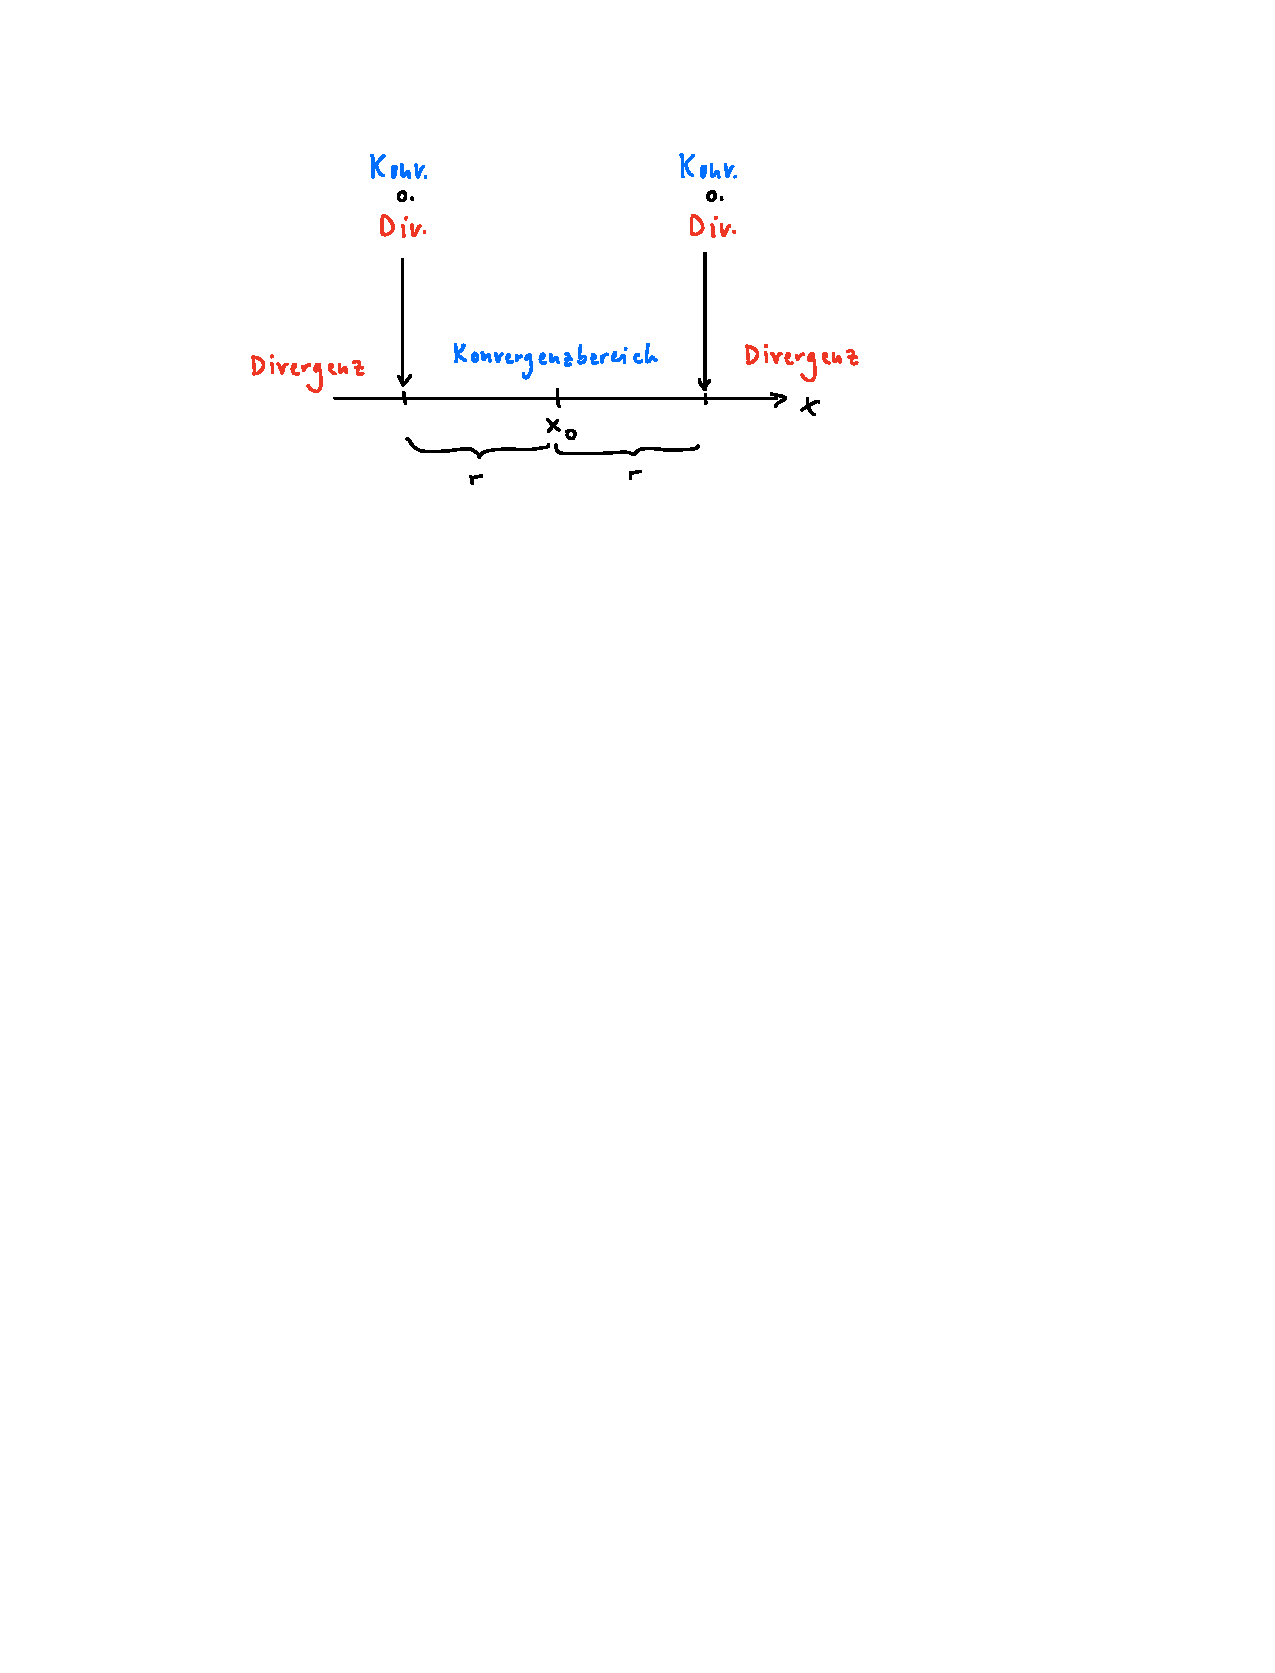
\includegraphics[width=0.65\linewidth]{src/Potenzreihen/konvergenzradius.pdf}
    \end{center}
    Innerhalb vom Konvergenzbereich darf man Potenzreihen \textit{gliedweise}:
    \begin{itemize}
        \item addieren \& subtrahieren
        \item integrieren \& differenzieren
    \end{itemize}
        % !TeX root = ../../ZF_bmicha_Ana.tex
\subsection{Taylorreihen}
    Taylorentwicklung von $f(x)$ um $x_o$:
    \mathbox{
        f(x) = \sum_{n=0}^\infty \frac{f^{(n)}(x_o)}{n!} (x-x_o)^n
    }
    \begin{itemize}
    \item ungerade Fkt $\Leftrightarrow$ ungerade Indizes: $a_1x + a_3x^3 + \dots$
    \item gerade Fkt $\Leftrightarrow$ gerade Indizes: $a_0 + a_2x^2 + \dots$
    \end{itemize}
    
    \vspace{3pt}
    
    \subsubsection{Taylorriehenentwicklung einer DGL}
    \vspace{3pt}
    \fcolorbox{black}{white}{\parbox{0.95\linewidth}{Es existiert höchstens eine Potenzreihe von $f$ um $x_o$. \\ $\Rightarrow$ lässt sich eine Taylorreihe bilden, so entspricht sie der Potenzreihe der Funktion an der Stelle $x_o$}} \vspace{3pt}
    
    \textit{gegeben: DGL, Anfangsbedingung \\ gesucht: Potenzreihenentwicklung um $x_o$, n Koeff. }
    \begin{enumerate}
        \item die ersten $(n-1)$ Ableitungen bilden, keine Terme höher als $x^n$ 
        $$y(x) = a_o + a_1x + a_2x^2 + a_3x^3 + ... $$
        $$y'(x) = a_1 + 2a_2x + 3a_3x^2 + ... $$
        $$ y''(x) = 2a_2 +  6 a_3x + 12a_4x^2 + ...$$
        \item Anfangsbedingung einsetzen und Werte für $y, y', y'', ...$ finden 
        \item Werte in die allgemeine Form einsetzen: 
        $$y(x) = y(x_o) + \frac{y'(x_o)}{1!}(x-x_o) + \frac{y''(x_o}{2!}(x-x_o)^2 + ... $$
    \end{enumerate}
    \newpage 
        \section{Appendix}
        \subsection{Trigonometrie \texorpdfstring{ \hfill S.97-99}{S.97-99}}
\vspace{2pt}
        %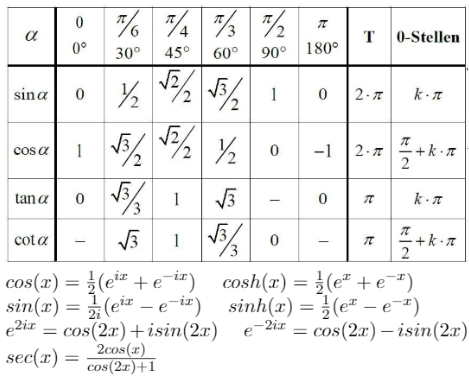
\includegraphics[width= \linewidth]{src/Appendix/Standardwerte_Trigonometrie.png}
\renewcommand{\arraystretch}{2}
$
\begin{array}{|l||c|c|c|c|c|c||c|c|}
    \hline
    \textrm{rad} & 0 & \frac{\pi}{6} & \frac{\pi}{4} & \frac{\pi}{3} & \frac{\pi}{2} & \pi & \textrm{\textbf{T}} & \textrm{\textbf{Nst.}}  \\
    \grad & 0^o & 30^o & 45^o & 60^o & 90^o & 180^o & &  \\
    \hline 
    \sin\alpha & 0 & \frac{1}{2} & \frac{\sqrt{2}}{2} & \frac{\sqrt{3}}{2} & 1 & 0 & 2\pi & k\!\cdot\!\pi \\
    \hline 
    \cos{\alpha} & 1 & \frac{\sqrt{3}}{2} & \frac{\sqrt{2}}{2} & \frac{1}{2} & 0 & -1 & 2\pi & \frac{\pi}{2}\!+\!k\!\cdot \!\pi \\
    \hline 
    \tan \alpha & 0 & \frac{\sqrt{3}}{3} & 1 & \sqrt{3} & - & 0 & \pi & k\!\cdot \! \pi \\
    \hline 
    \cot \alpha & - & \sqrt{3} & 1 & \frac{\sqrt{3}}{3} & 0 & - & \pi & \frac{\pi}{2}\!+\!k\!\cdot \!\pi \\
    \hline 
\end{array}
$

\begin{align*}
    \cos x &= \frac{1}{2}(e^{ix} + e^{-ix}) & \cosh x &= \frac{1}{2}(e^x + e^{-x}) \\
    \sin x &= \frac{1}{2i}(e^{ix} - e^{-ix}) & \sinh x &= \frac{1}{2}(e^x - e^{-x} \\
    e^{2ix} &= \cos(2x)\!+\! i\sin(2x) & e^{-2i} &= \cos(2x)\!-\!i\sin(2x) \\
    \sec x &= \frac{2 \cos x}{\cos(2x) + 1} && \\ 
\end{align*}

%\subsection{Koordinatentransformation}
%        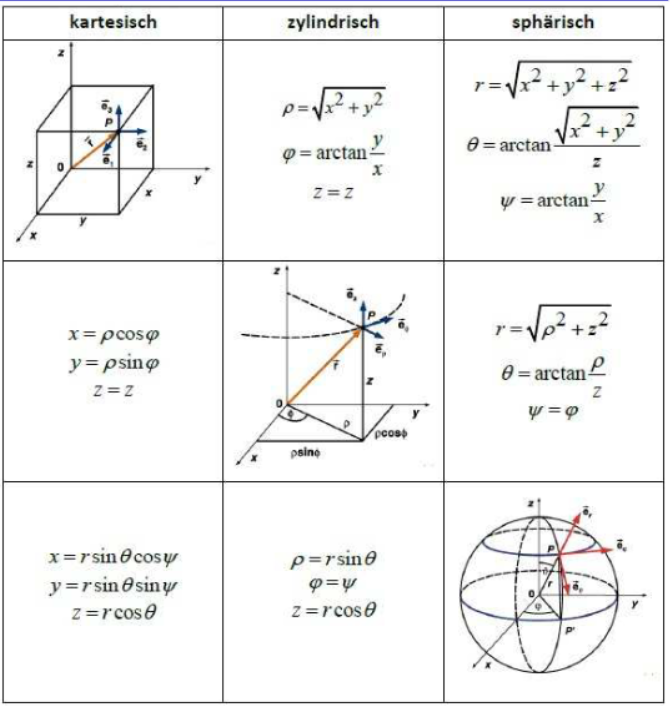
\includegraphics[width = \linewidth]{src/Appendix/Koordinatentransformation.png}
%        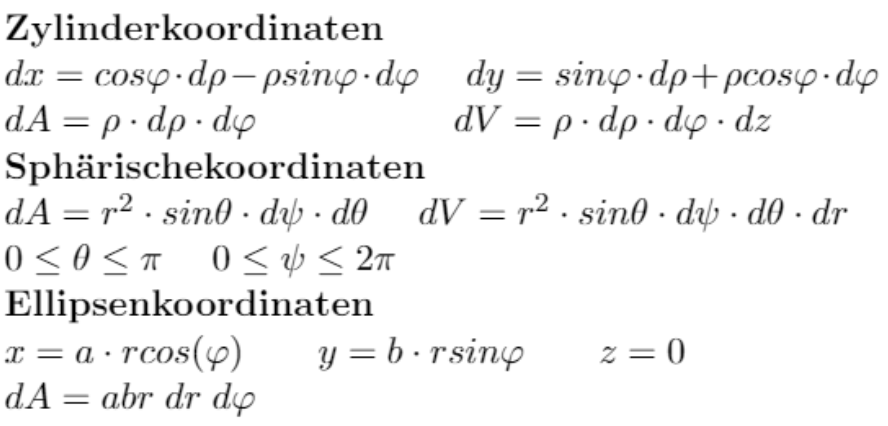
\includegraphics[width = \linewidth]{src/Appendix/Formel Koordinatentransformation.png}
% !TeX root = ../../ZF_bmicha_Ana.tex
\subsection{Cosinus und Sinus - Integrale \texorpdfstring{\hfill S.74}{S.74}}
    
    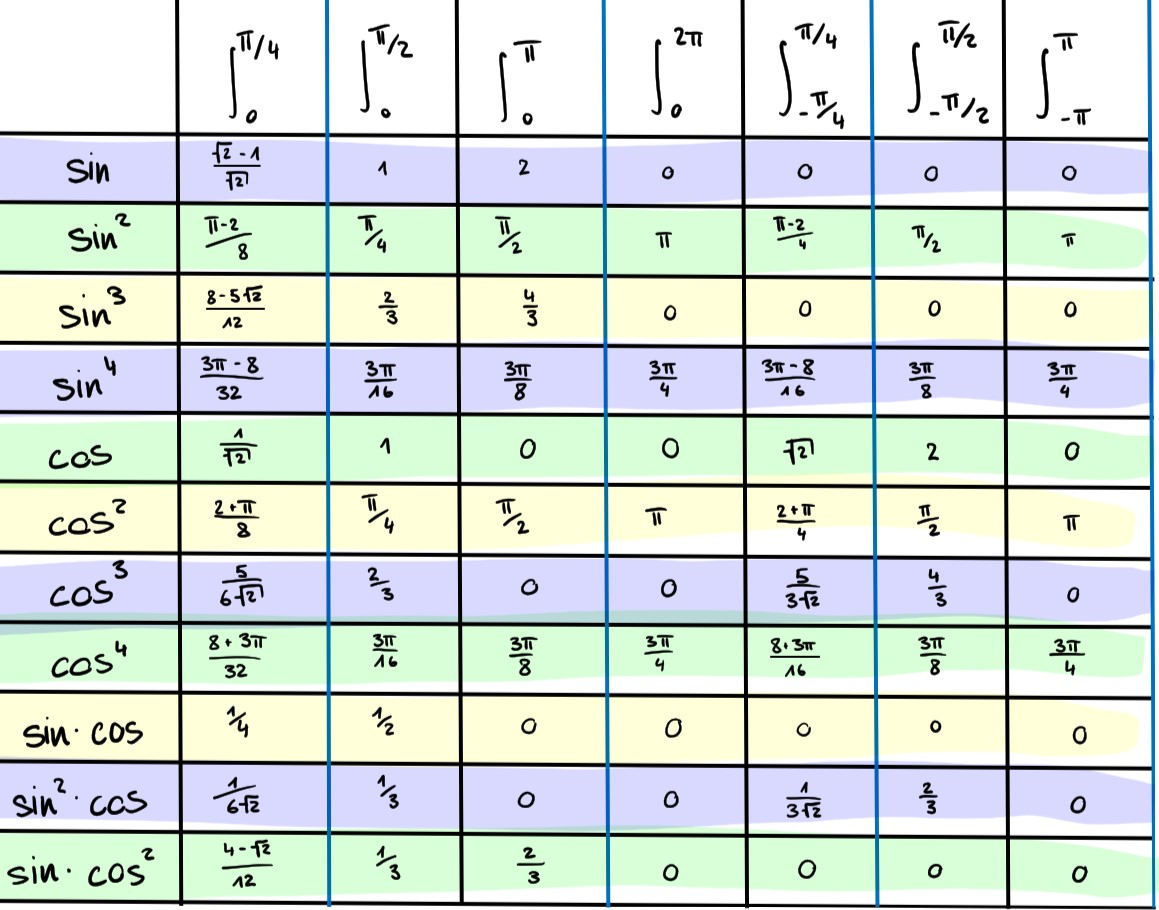
\includegraphics[width = \linewidth]{src/Appendix/integraltabelle_sin_cos.jpg}
    Für $a,b \in \mathbb{N}$ und $n \geq 2$, gelten:
    \begin{align*}
        \int_{a \cdot \frac{\pi}{2}}^{b \cdot \frac{\pi}{2}} \sin^n(x) \ dx 
            &= \frac{n-1}{n} \int_{a \cdot \frac{\pi}{2}}^{b \cdot \frac{\pi}{2}} \sin^{n-2}(x) \ dx\\[0.5em]
        \int_{a \cdot \frac{\pi}{2}}^{b \cdot \frac{\pi}{2}} \cos^n(x) \ dx 
            &= \frac{n-1}{n} \int_{a \cdot \frac{\pi}{2}}^{b \cdot \frac{\pi}{2}} \cos^{n-2}(x) \ dx
    \end{align*}

\subsection{Ableitungsregeln \texorpdfstring{\hfill S.62-65}{S.62-65}}
        
        Kettenregel 
       $$[f(x) \cdot  g(x)]' = f'(x)\cdot g(x) + f(x) \cdot  g'(x)$$
       Quotientenregel
       $$ [\frac{f(x)}{g(x)}]' = \frac{f'(x)\cdot g(x) - f(x)\cdot g'(x)}{g^2(x)} $$
       Verallgemeinerte Kettenregel
       $$F'(x(t), y(t)) = f_x (x(t), y(t)) \cdot  \dot{x} + f_y (x(t), y(t)) \cdot  \dot{y} $$
       
\subsection{Additionstheoreme \texorpdfstring{\hfill S.99}{S.99}}
    \textbf{$\textrm{cot} = \textrm{tan}^{-1}$}
    \begin{align*}
            1 + cot^2(x) = \frac{1}{sin^2(x)} && cot(a \pm b) = \frac{cot(a)cot(b) \mp 1}{cot(a) \pm cot(b)} \\
            cot(2a) = \frac{cot^2(a) -1}{2 cot(a)}
    \end{align*}
    \textbf{a/2}
    $$ sin \left( \frac{a}{2} \right) = \pm \sqrt{\frac{1}{2}\cdot (1-cos(a)} $$
    $$ cos \left( \frac{a}{2} \right) = \pm \sqrt{\frac{1}{2}\cdot (1+cos(a)} $$

\subsection{Integrationsregeln \texorpdfstring{\hfill S.70-72}{S.70-72}}
       $$ \frac{d}{dx} \int_a^{u(x)} f(u) du = f(g(x)) * g'(x)$$
       Partielle Integration: 
       $$ \int u'\cdot v dx = u\cdot v - \int u\cdot v' dx $$
       Substitution 1. Art \vspace{2pt}
       \begin{center}
           $ \int_a^b f(u(x))u'(x) dx = \int_{u(a)}^{u(b)} f(z) dz $, wobei $ z = u(x)$
       \end{center}
       
       Substitution 2. Art \vspace{2pt}
       \begin{center}
           $ \int_a^b f(x) dx = \int_{u(a)}^{(u(b)} f(u(z))\cdot u'(z) dz $, wobei $ x = u(z)$
       \end{center}

\subsection{Partialbruchzerlegung, Polynomfkt. \texorpdfstring{\hfill S.21+57}{S.21+57}}
        \vspace{3pt}
       \begin{enumerate}
           \item einfache Nullstelle: $ \frac{A}{x - x_0}$
           \item doppelte Nullstelle: $\frac{A}{x - x_0} + \frac{B}{(x-x_0)^2} $
           \item komplexe Nullstelle: $ \frac{A*x + B}{(z.B.: x^2 + 1)}$
       \end{enumerate}

\subsection{Komplexe Zahlen \texorpdfstring{\hfill S.18-19}{S.18-19}}
       \vspace{3pt}
       
       \def\arraystretch{1.5}
       \begin{tabular*}{\linewidth}{ll}
           imaginäre Einheit: & $i^2 = 1$ \\
           Normalform: & $ z = a + ib $ \\
           Polarform: & $ z = r(cos\phi + isin\phi) $ \\
           Exponentialform: & $ z = re^{i\phi} $ \\
           Konjugierte: & $ \bar{z} = a\!-\!ib = r(cos\phi\!-\!isin\phi) = re^{-i\phi} $
       \end{tabular*}
       \vspace{5pt}
       
       Winkel grösser als $2\pi$ können auf ihr Äquivalent im Bereich $[0; 2\pi]$ reduziert werden \\[3pt]
       Form: $\arg (z) = \phi = \textrm{Winkel}$ \vspace{6pt}
       
       \textbf{Umrechnungsformeln:}
       
       \vspace{3pt}
       
       \begin{tabular*}{\linewidth}{ll}
           Normal- $\rightarrow$ Polarform: & $ r = \sqrt{a^2 + b^2} $ \\
           & $ cos\phi = \frac{a}{r}, sin\phi = \frac{b}{r} $ \\
           Polar- $\rightarrow$ Normalform: & $ a = rcos\phi, b = rsin\phi $
       \end{tabular*}
       
       \vspace{5pt}
       
       \textbf{Operationen siehe S.18}\\[3pt]
       \textit{Hinweis: bei Multiplikation einer kompl. Zahl mit Betrag 1 dann wird um den Ursprung rotiert.} \vspace{5pt}
       
       \cbreak
       
       \textbf{Potenzieren:}
       
       $$z^n = r^n e^{in\phi} $$
       
       \textbf{Wurzel ziehen:}
       
       Sucht man $n$ Wurzeln $w$ der komplexen Zahlen $z$, so setzt man $k = 0, 1,..,n-1$ in die folgende Fomrel ein: 
       $$ w_k = \sqrt[k]{|z|} \cdot e^{i(\frac{\phi}{k} + \frac{2\pi k}{k})} $$

       \begin{minipage}{0.49\linewidth}
           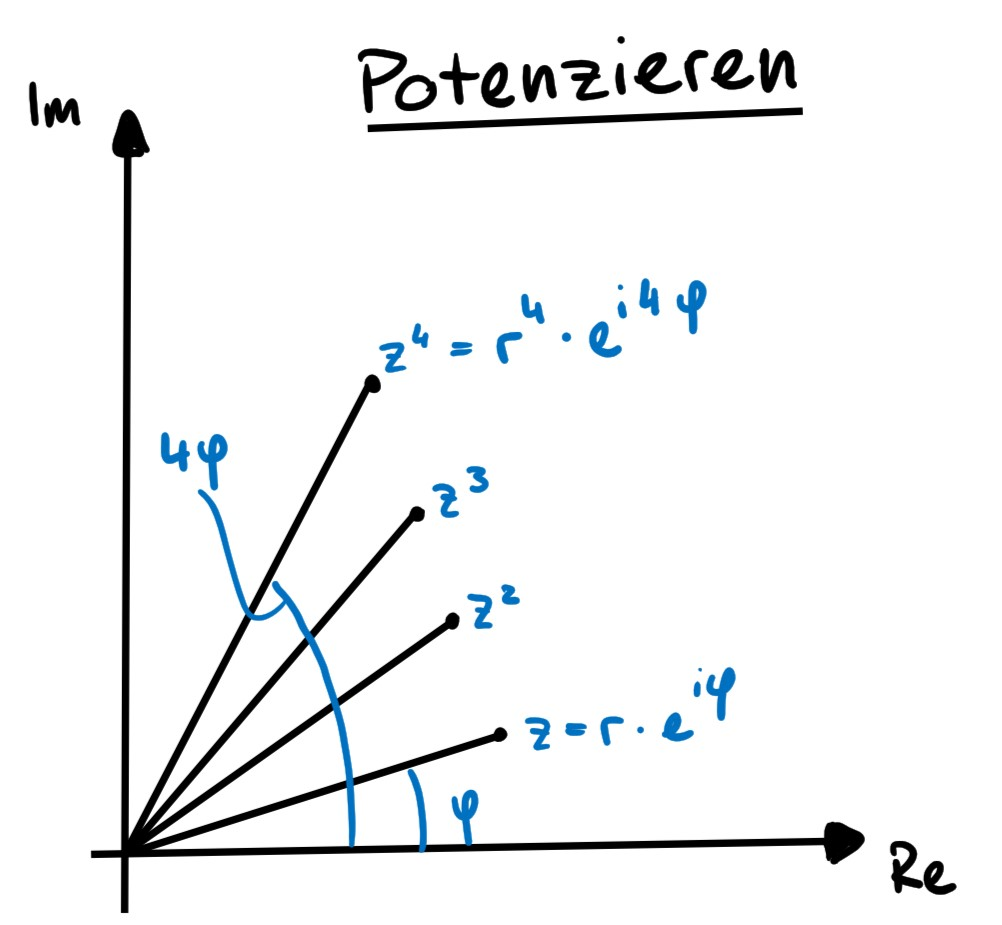
\includegraphics[width=\linewidth]{src/Appendix/1_komplexe_Zahlen_potenzieren.jpg}
       \end{minipage}
       \begin{minipage}{0.5\linewidth}
        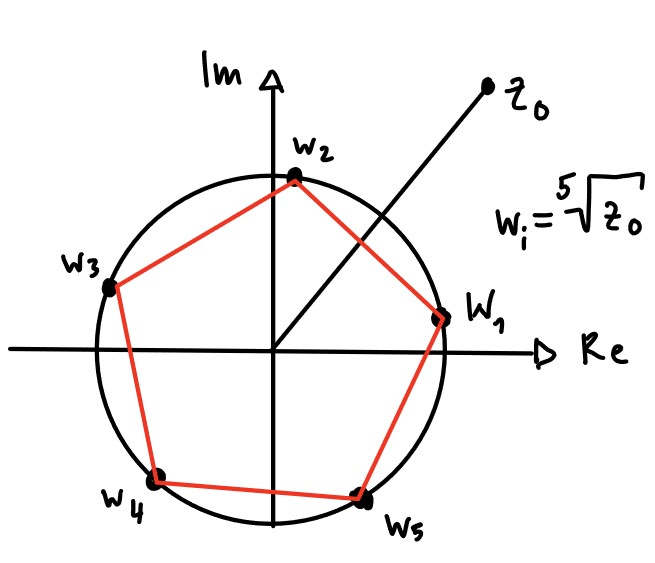
\includegraphics[width= \linewidth]{src/Appendix/kompl_Zahlen_wurzeln.jpg}
       \end{minipage}
        % !TeX root = ../../ZF_bmicha_Ana.tex
\subsection{Nullstellen Reeller Polynome mit Grad \texorpdfstring{$n$}{n}}
    %\vspace{-1em}
    $$
        p(x) = a_0 + a_1 x + a_2 x^2 + \dots + a_n x^n, \qquad a_i \in \mathbb{R}
    $$
    \begin{itemize}
        \item Hat genau $n$ Nullstellen (komplex und reell)
        \item Komplexe Nullstellen kommen immer im komplex-konjugierten Paar vor.
    \end{itemize}
        \subsection{Integrale aus Vorlesung \texorpdfstring{\hfill S.72-74 + S.65}{S.72-74 + S.65}}
\vskip3pt
\small{
$ 
\int x(ax+b)^n dx = \frac{(ax + b)^{n+2}}{(n+2)a^2} - \frac{b(ax + b)^{n+1}}{(n+1)a^2} \\[6pt]
\int \frac{x}{(ax+b)^n} dx  = - \frac{1}{(n-2)a^2 (ax+b)^{n-2}} + \frac{b}{(n-1)a^2 (ax + b)^{n-1}} \\[6pt]
\int x^2 (ax+ b)^n dx = \frac{(ax+b)^{n+3}}{(n+3)a^3} - \frac{2b(ax+b)^{n+2}}{(n+2)a^3} + \frac{b^2 (ax+b)^{n-1}}{(n+1)a^3} \\[6pt]
\int \frac{x}{ax^2 + b} dx = \frac{1}{2a} ln|ax^2 + b| \\[6pt]
\int \frac{x}{(a^2 + x^2)^n} dx = \frac{-1}{2(n-1)(a^2 + x^2)^{n-1}} \\[6pt]
\int \frac{x}{(a^2 - x^2)^n} dx = \frac{1}{2(n-1)(a^2 - x^2)^{n-1}} \\[6pt]
\int \frac{x}{x^4 + 3} dx = \frac{\sqrt{3}}{6} arctan(\frac{x^2}{\sqrt{3}}) \\[6pt]
\int \frac{x}{\sqrt{x^2 + 1}} dx = \sqrt{x^2 + 1} \\[6pt]
\int \frac{x}{x^2 + y^2} dy = arctan(\frac{y}{x}) \\[6pt]
\int \frac{-y}{x^2 + y^2} dx = arctan(\frac{y}{x})  \\[6pt]
\int \frac{x^2 - y^2}{x^2 + y^2} dx = \frac{y}{x^2 + y^2}  \\[6pt]
\int \frac{1}{x^2 + a^2} dx = \frac{1}{a} arctan(\frac{x}{a}) \hskip3pt a \neq 0  \\[6pt] 
\int \frac{1}{x^2 - a^2} dx = \frac{1}{2a} ln(\frac{x-a}{x+a}) \\ [6pt]
\int \frac{1}{x^2 + x} dx = ln(x) - ln(x+1) \\[6pt]
\int \frac{1}{1+x^2} dx = arctan(x) \\[6pt]
\int_{-\infty}^{\infty} \frac{1}{1 + x^2} dx = \pi \\[6pt]
\int \frac{1}{1-x^2} dx = artanh(x) = ln(\sqrt{\frac{1+x}{1-x}}) |x| < 1 \\[6pt]
\int \frac{1}{ax^2 + bx + c} dx = \frac{2arctan(\frac{2ax+b}{\sqrt{4ac - b^2}})}{\sqrt{4ac-b^2}} \\[6pt]
\int \frac{1}{(x^2 + x -6 )} dx = \frac{1}{5} ln \left( \frac{x-2}{x+3} \right) \\[6pt]
\int \frac{1}{x^2 + x + 1} dx = \frac{2}{\sqrt{3}} arctan \left( \frac{2x+1}{\sqrt{3}} \right) \\[6pt]
\int \frac{1}{\sqrt{x^2 + 1}} dx = arsinh(x) = ln(x + \sqrt{x^2 + 1}) \\[6pt]
\int \frac{1}{\sqrt{x^2 - 1}} dx = arcosh(x) = ln(x + \sqrt{x^2 -1}) \hskip3pt 1 \leqslant x \\[6pt]
\int \frac{1}{\sqrt{1-x^2}} dx = arcsin(x) = -arccos(x) \\[6pt]
\int \sqrt{1+x^2} dx = \frac{1}{2} \left( arsinh(x) + x \cdot \sqrt{1+x^2} \right) \\[6pt]
\int \sqrt{1-x^2} dx = \frac{1}{2} \left( arcsin(x) + x \cdot \sqrt{1-x^2} \right) \\[6pt]
\int x^2 \cdot sin(x) dx = -x^2cos(x) + 2sin(x) - 2 cos(x) \\ [6pt]
\int x \cdot sin(ax) dx = \frac{1}{a^2} sin(ax) - \frac{x}{a} cos(ax) \\[6pt]
\int \frac{x}{sin^2(x)} dx = -x \cdot cot(x) + ln(sin(x)) \\ [6pt]
\int \frac{1}{sin^2(x)} dx = -cot(x) = tan(x + \frac{\pi}{2}) \\[6pt]
\int \frac{1}{cos^2(x)} dx = tan(x) \\[6pt]
\int sin^2(x) dx = \frac{1}{2} \left( x - sin(x)cos(x) \right)) \\[6pt]
\int sin^3(x) dx = \frac{1}{12} (cos(3x) - 9 cos(x)) \\[6pt]
\int sin^4(x) dx = \frac{1}{32} (12x - 8sin(2x) + sin(4x)) \\[6pt]
\int cos^2(x) dx = \frac{1}{2} (x + sin(x)cos(x)) \\[6pt]
\int cos^3(x) dx = sin(x) - \frac{sin^3(x)}{3} = \frac{1}{12}(9sin(x) + sin(3x)) \\[6pt]
\int cos^4(x) dx = \frac{1}{32}(12x + 8sin(2x) + sin(4x)) \\[6pt]
\int sin^{3/2}(2x) dx = -\frac{1}{2} cos(2x) \\[6pt]
\int cos^{3/2}(2x) dx = sin(x)cos(x) \\[6pt]
\int cos(2x)dx = \frac{1}{2} sin(2x) \\[6pt]
\int sin(x)cos(x) dx = -\frac{1}{2} cos^2(x) \\[6pt]
\int sin^2(x) cos(x) dx = \frac{1}{3}sin^3(x) \\[6pt]
\int sin(x)cos^n(x) dx = - \frac{1}{n+1} cos^{n+1}(x) \hspace{3pt} n \geqslant 0\\[6pt]
$
}
    \cbreak
        \subsection{einige wichtige Kurven \texorpdfstring{\hfill S.55 / 67}{S.55 /67}}
\vspace{3pt}
\subsubsubsection{Kreis mit Mittelpunkt $(x_o, y_o)$ und Radius $R$} 
\vspace{3pt}
\begin{minipage}{0.5\linewidth}
        \vspace{0.5em}
        \textit{implizit:}
        $$
            (x - x_o)^2  + (y - y_o)^2 = R^2
        $$
        \textit{parametrisiert:}
        \begin{align*}
            x &= x_o + R\cos{t}\\
            y &= y_o + R\sin{t}\\
        \end{align*}
\end{minipage}
\begin{minipage}{0.49\linewidth}
        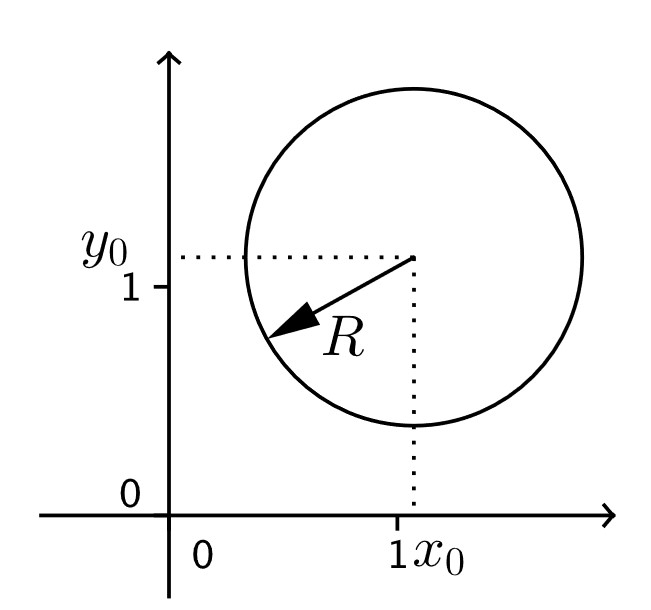
\includegraphics[width=0.8\linewidth]{src/Appendix/Kreis.jpg}
\end{minipage}
    
\subsubsubsection{Ellipse mit Mittelpunkt $(x_o, y_o)$ und Halba. $a, b$}
\vspace{3pt}
\begin{minipage}{0.5\linewidth}
        \vspace{0.5em}
        \textit{implizit:}
        $$
            \frac{(x - x_o)^2}{a^2}  + \frac{(y - y_o)^2}{b^2} = 1
        $$
        \textit{parametrisiert:}
        \begin{align*}
            x &= x_o + a\cos{t}\\
            y &= y_o + b\sin{t}\\
        \end{align*}
\end{minipage}
\begin{minipage}{0.49\linewidth}
        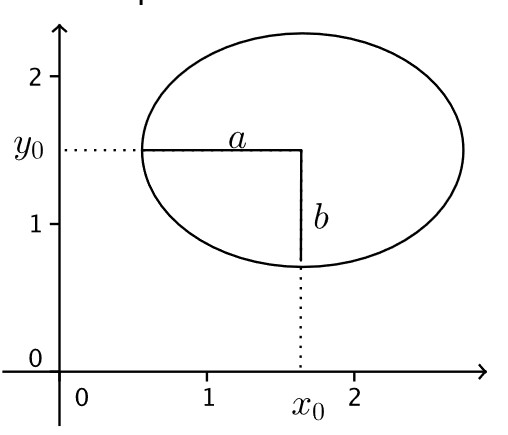
\includegraphics[width=0.8\linewidth]{src/Appendix/Ellipse.jpg}
\end{minipage}

\subsubsubsection{Hyperbel 1 \texorpdfstring{\hfill S.108}{S.108}}
\vspace{3pt}
\begin{minipage}{0.5\linewidth}
        \vspace{0.5em}
        \textit{implizit:}
        $$
            \frac{x^2}{a^2}  - \frac{y^2}{b^2} = 1
        $$
        \textit{parametrisiert:}
        \begin{align*}
            x &= \pm a \cosh{t}\\
            y &= b \sinh{t}\\
        \end{align*}
\end{minipage}
\begin{minipage}{0.49\linewidth}
        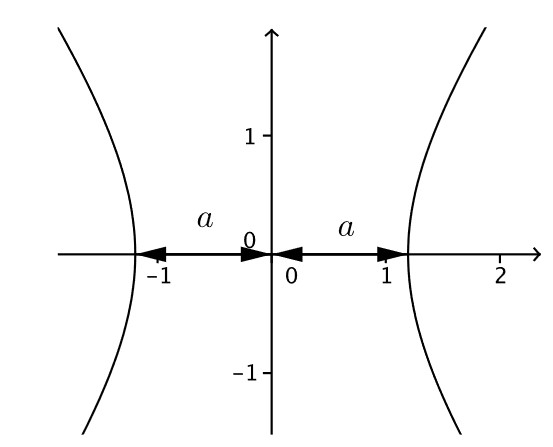
\includegraphics[width=0.8\linewidth]{src/Appendix/Hyperbel.jpg}
\end{minipage}

\subsubsubsection{Hyperbel 2}
\vspace{3pt}
\begin{minipage}{0.5\linewidth}
        \vspace{0.5em}
        \textit{explizit:}
        $$
            y = \frac{a}{x}
        $$
        \textit{parametrisiert:}
        \begin{align*}
            x &= t\\
            y &= \frac{a}{t}\\
        \end{align*}
\end{minipage}
\begin{minipage}{0.49\linewidth}
        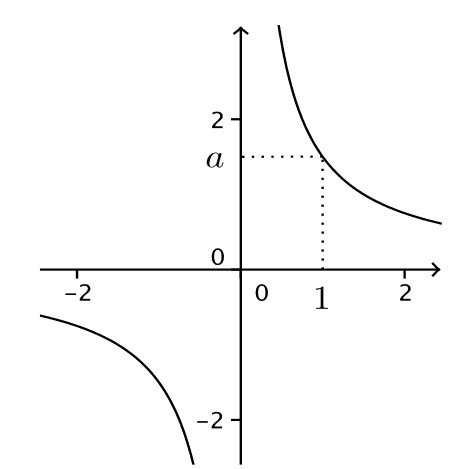
\includegraphics[width=0.8\linewidth]{src/Appendix/Hyperbel 2.jpg}
\end{minipage}



\end{document}